\documentclass[10pt]{beamer}

%\usepackage{eulervm}

%\usefonttheme[onlymath]{professionalfonts}
\usetheme[progressbar=frametitle]{metropolis}
\usepackage{appendixnumberbeamer}

\usepackage{booktabs}
\usepackage[scale=2]{ccicons}

\usepackage{pgfplots}
\usepgfplotslibrary{dateplot}
\usepgfplotslibrary{fillbetween}
\usetikzlibrary{calc}

\usepackage{xspace}
\newcommand{\themename}{\textbf{\textsc{metropolis}}\xspace}

\usepackage{amsmath,amssymb}
\newcommand{\mat}[1]{\ensuremath{\boldsymbol{{#1}}}}
\newcommand{\mel}[1]{\ensuremath{{{#1}}}}
\newcommand{\phym}[1]{\ensuremath{\mathsf{#1}}}

\newcommand{\inlinebar}[2]{\begin{tikzpicture}
    \begin{axis}[
        grid=major,
        width=40mm,
        height=20mm,
        scale=1,
        xmin=0, xmax=1.2, ymin=0, ymax=1,
        xtick = {0,1}, ytick = {0.,1},
        xmajorticks=false,
        ymajorticks=false]
     \addplot[fill=#2, fill opacity=.3, draw=none, samples=500]
       plot (\x, {sign(#1-\x) } );
   \end{axis}
\end{tikzpicture}}


\newcommand{\inlineprob}[3]{\begin{tikzpicture}
    \begin{axis}[
        grid=major,
        width=40mm,
        height=20mm,
        scale=1,
        xmin=0, xmax=1.2, ymin=0, ymax=1,
        xtick = {0,1}, ytick = {0.,1},
        %xticklabel={\pgfmathparse{\tick*100}\pgfmathprintnumber{\pgfmathresult}\%},
        xmajorticks=false,
        ymajorticks=false]
     \addplot[fill=#3, fill opacity=.3, samples=500, draw=none]
       plot (\x, {1/(1+exp((\x-#1)*#2))} ) \closedcycle;
   \end{axis}
\end{tikzpicture}}

\newcommand{\TikzCross}{\mathbin{\tikz [x=1.4ex,y=1.4ex,line width=.2ex, red] \draw (0,0) -- (1,1) (0,1) -- (1,0);}}%

\definecolor{darkgreen}{rgb}{.1, .8, .1}
\newcommand{\Checkmark}{\color{darkgreen}\checkmark}
\definecolor{renewablegreen}{rgb}{.1, .7, .1}

\newcommand{\graafjeduitsland}[9]{
\begin{tikzpicture}[scale=.6]
    \node[draw, circle](b) at (6,3){#1};
    \node[draw, circle](h) at (0,6){#2};
    \node[draw, circle](f) at (1,2){#3};
    \node[draw, circle](l) at (5,0){#4};
    \node[above, opacity=.6] at ($(b.north) + (.3,.1)$) {\emph{Berlin   }};
    \node[above, opacity=.6] at (h.north) {\emph{Hamburg  }};
    \node[below, opacity=.6] at ($(f.south) - (.6,.1)$) {\emph{Frankfurt}};
    \node[below, opacity=.6] at (l.south) {\emph{Leipzig  }};
    
    \draw[-latex] (b) -- node[midway, left] {#5} (l);
    \draw[-latex] (l) -- node[midway, above]{#6} (f);
    \draw[-latex] (f) -- node[midway, above]{#7} (b);
    \draw[-latex] (b) -- node[midway, above]{#8} (h);
    \draw[-latex] (h) -- node[midway, right]{#9} (f);
\end{tikzpicture}
}

\newcommand{\tododot}{\hspace{.5mm}{\tikz{\node[circle,fill=accentje,scale=.5] {}}}}
\newcommand{\maybetododot}{\hspace{.5mm}{\tikz{\node[circle,draw=accentje,scale=.5] {}}}}

\newcommand\blfootnote[1]{%
  \begingroup
  \renewcommand\thefootnote{}\footnote{#1}%
  \addtocounter{footnote}{-1}%
  \endgroup
}

\newcommand{\plaatjeframe}{{\setbeamercolor{palette primary}{fg=black, bg=white}
\begin{frame}[standout]
  \href{https://observablehq.com/@olivier_plas/cascading-line-failures-caused-by-renewable-fluctiations}{\texttt{fonsp.com/plaatje}}
\end{frame}
}}


% https://coolors.co/ed1c24-f5bb00-fdfffc-235789-020100
\definecolor{donker}{HTML}{0D2032}
\definecolor{accentje}{HTML}{F5BB00}
\definecolor{roodje}{HTML}{ED1C24}
\setbeamercolor{normal text}{fg=donker,bg=white}
\setbeamercolor{alerted text}{fg=roodje}


\title{Power Grid Failures - Renewable Energy}
\subtitle{How fluctuations in solar and wind affect grid security in Germany}
% \date{\today}
\date{\textit{July 2019}}
\author{\textbf{Fons van der Plas} \hfill \textit{supervisor:} Dr. Henk Don}
\institute{\texttt{f.vanderplas@student.ru.nl}}
% \titlegraphic{\hfill\includegraphics[height=1.5cm]{logo.pdf}}



\titlegraphic{%
    \hfill
\includegraphics[width=.3\textwidth]{img/ru_e_a4_cmyk_2014.eps}
}

\makeatletter
\setbeamertemplate{title page}{
    
  \begin{minipage}[b][\paperheight]{\textwidth}
    \vfill%
    \ifx\inserttitle\@empty\else{\vspace{2.5cm}\usebeamertemplate*{title}}\fi
    \ifx\insertsubtitle\@empty\else\usebeamertemplate*{subtitle}\fi
    \usebeamertemplate*{title separator}
    \ifx\beamer@shortauthor\@empty\else\usebeamertemplate*{author}\fi
    \ifx\insertdate\@empty\else\usebeamertemplate*{date}\fi
    \ifx\insertinstitute\@empty\else\usebeamertemplate*{institute}\fi
    \vfill
    \ifx\inserttitlegraphic\@empty\else\inserttitlegraphic\fi
    \vspace*{1cm}
  \end{minipage}
}
\makeatother



\begin{document}

{
\usebackgroundtemplate{\begin{tikzpicture}{\node[inner sep=0,outer sep=0, opacity=.1]{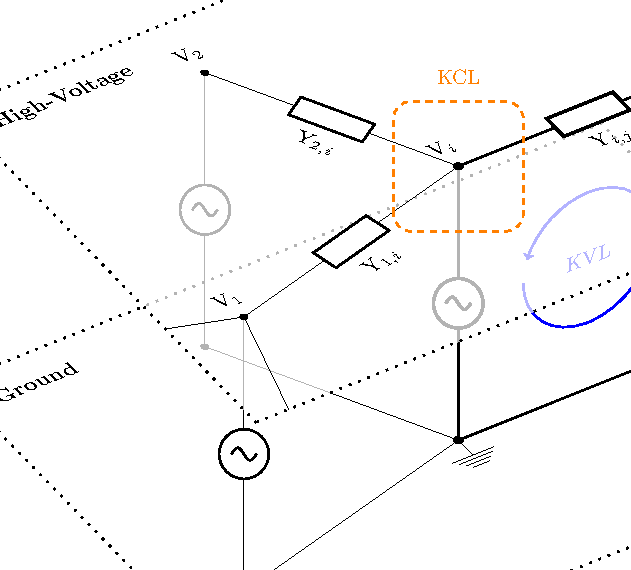
\includegraphics[width=\paperwidth]{img/vettegraafcrop2.pdf}};}\end{tikzpicture}}
\maketitle
}

{
\usebackgroundtemplate{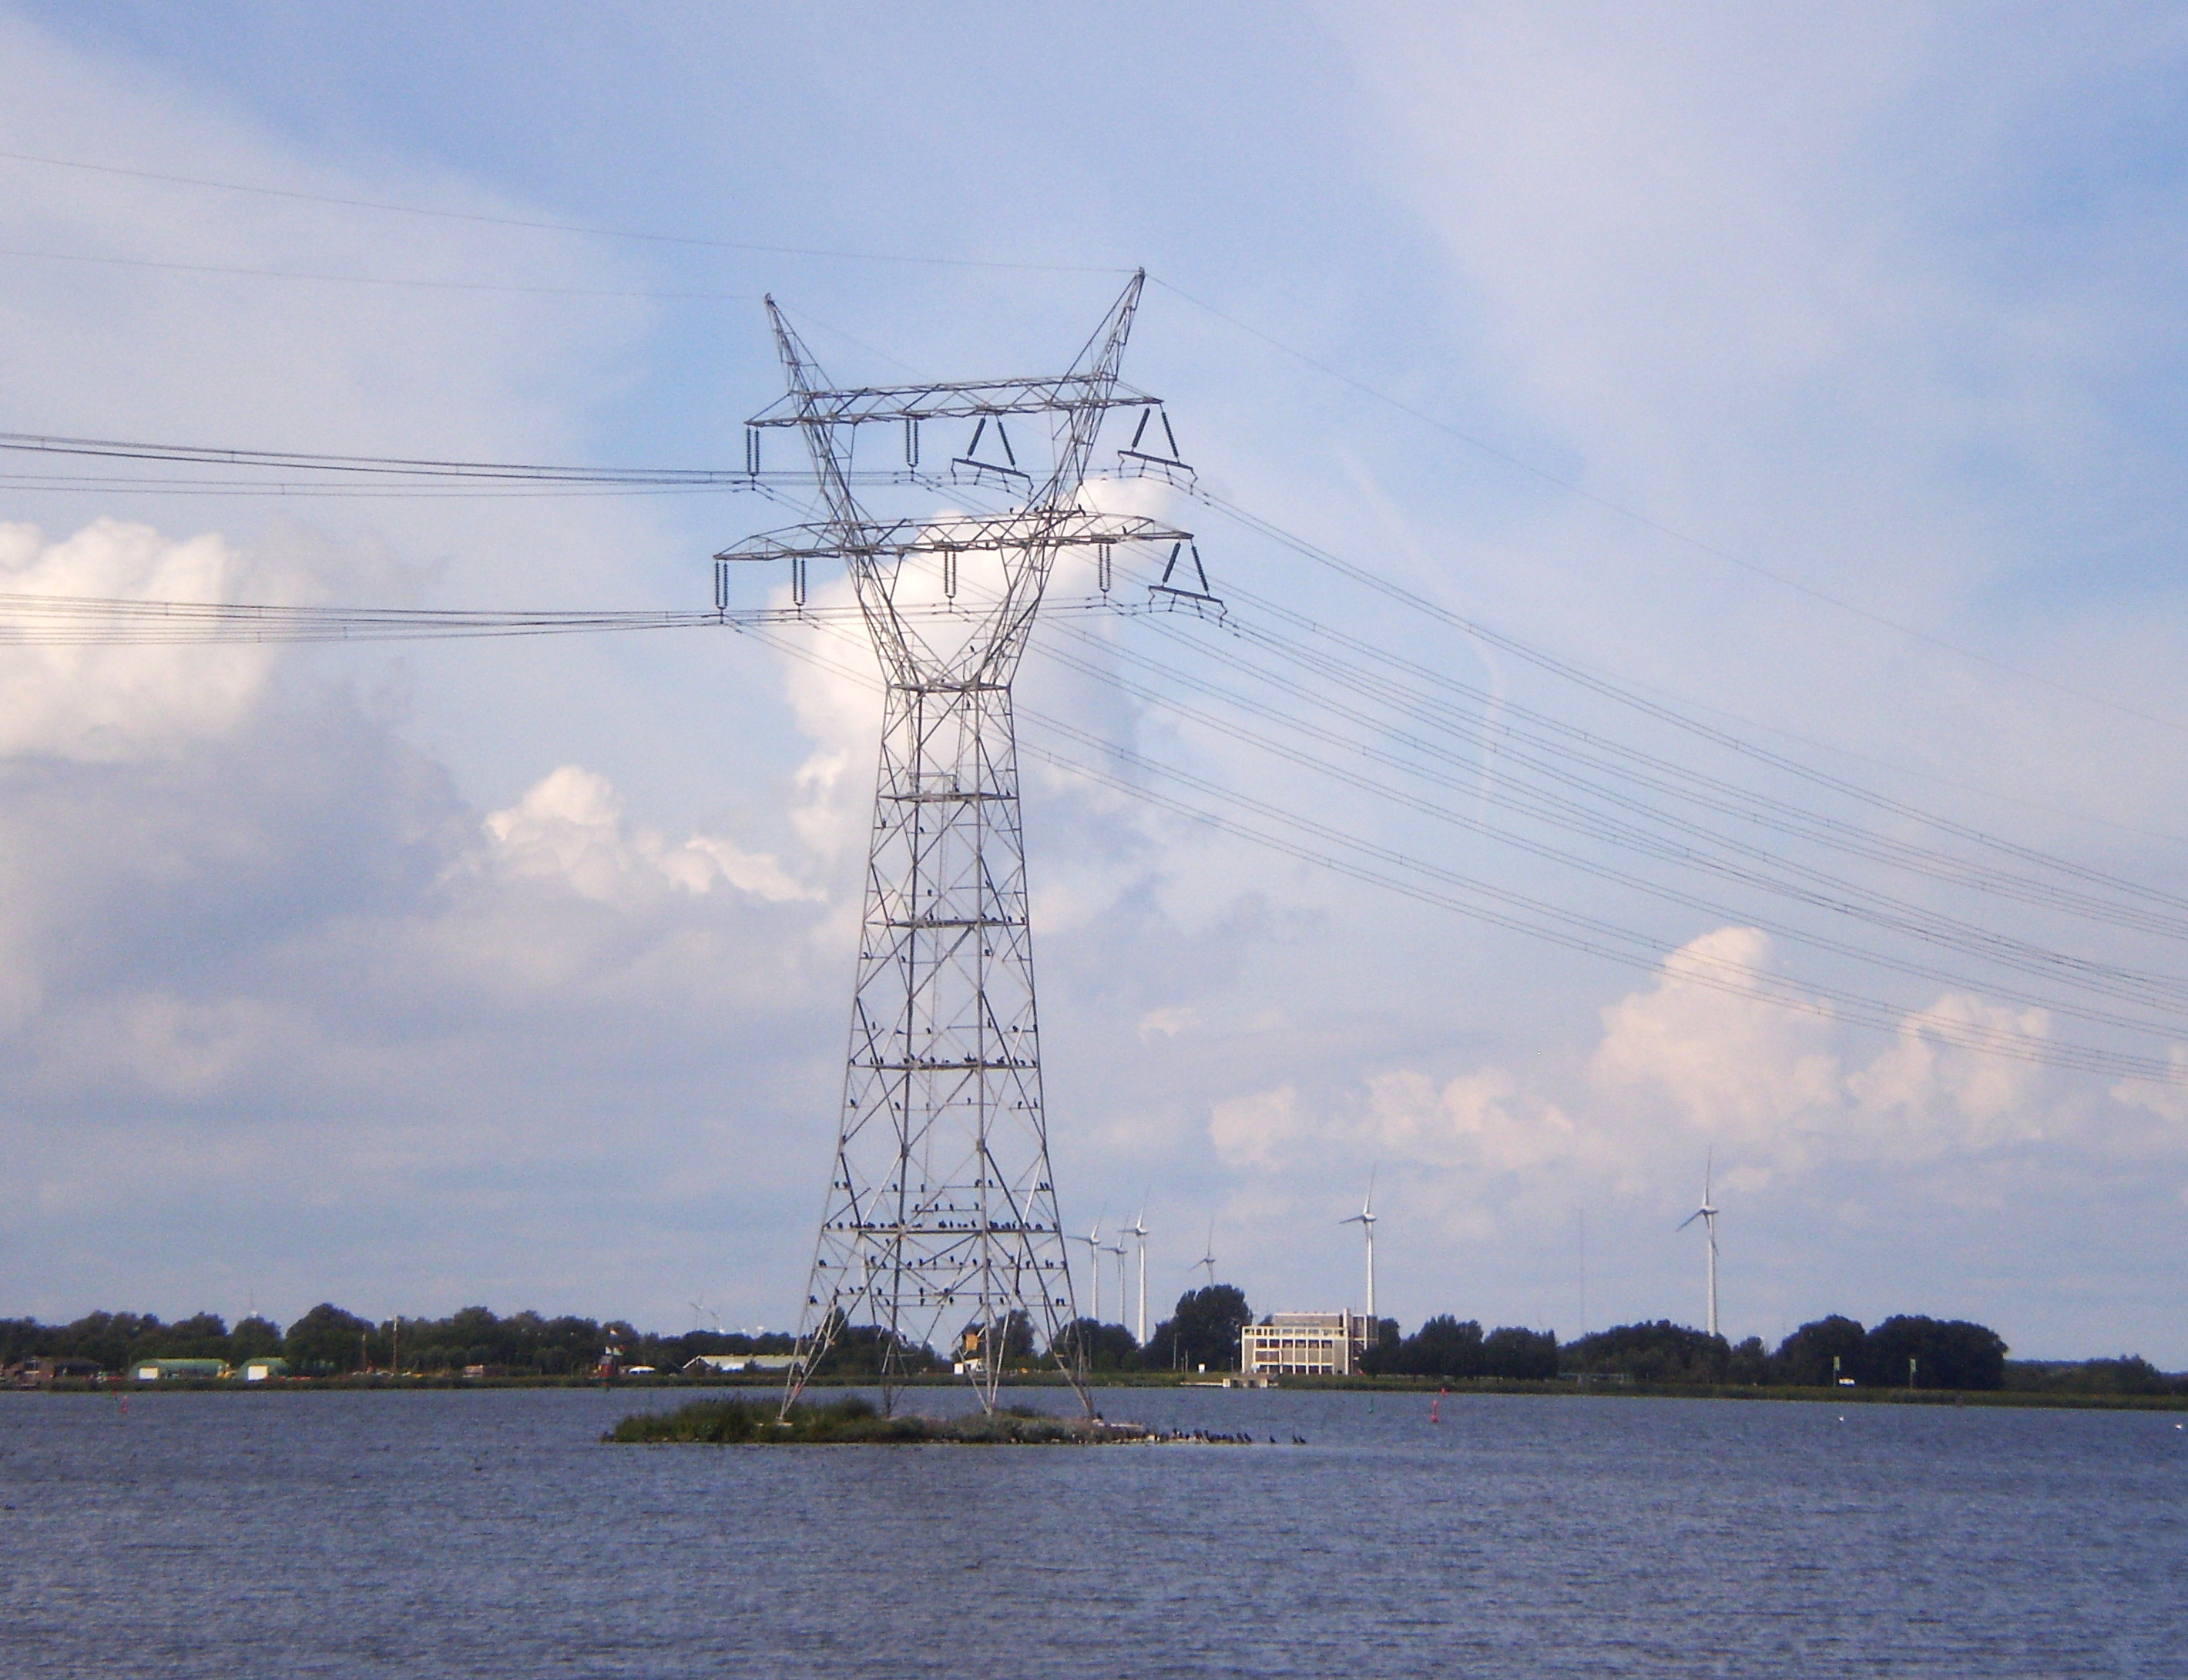
\includegraphics[width=\paperwidth]{img/Hoogspanningsmast_Veluwemeer.jpg}}
\setbeamertemplate{frame footer}{\color{white}{Wikimedia Commons}}
\setbeamertemplate{headline}{\vskip-\headheight}
\begin{frame}[noframenumbering]

\end{frame}
}

\begin{frame}{Transmission network of Germany}
    \begin{figure}
    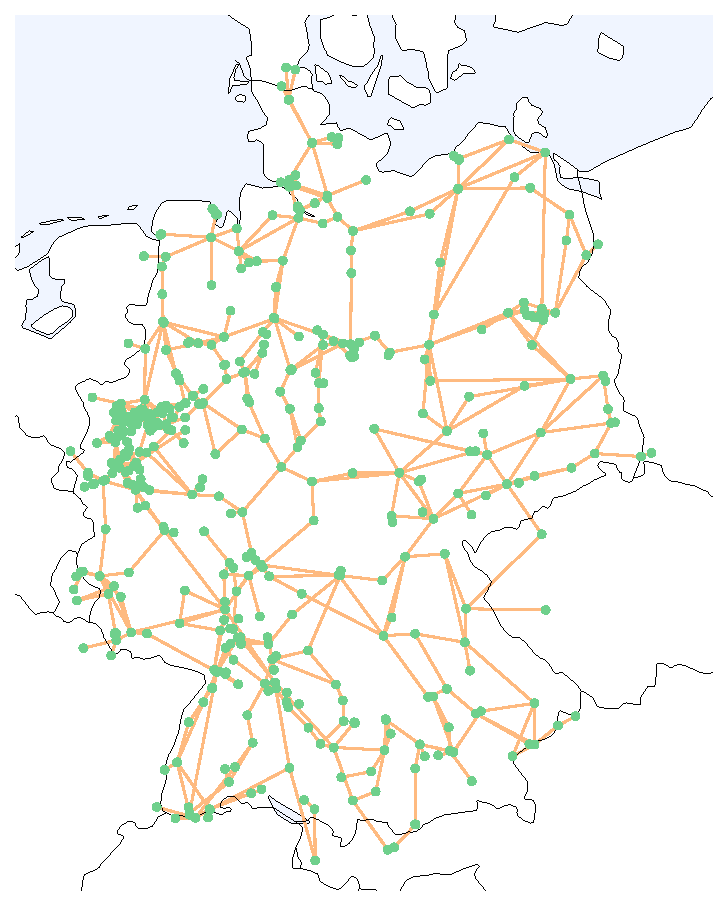
\includegraphics[height=.69\paperheight]{img/just_the_network.pdf}
    \caption{The $n=585$ nodes and $k=695$ lines of the SciGRID dataset.}
    \end{figure}
\end{frame}

\begin{frame}{Power injection}
    At each node $i\in\{1,\dots,n\}$:
    \[\mel{p}_i := S^{green}_i + S^{grey}_i - S^{load}_i\]
    \begin{table}[]
\begin{tabular}{l|ll}
\toprule
                         & \color{renewablegreen}{\textbf{green}} & \textbf{\textbf{grey}} \\
                         \midrule
\emph{Operation costs} & \textbf{0-10 €/MWh}       & 30-35 €/MWh      \\
\emph{CO2eq-emissions} & \textbf{0 kg/MWh}          & 490 - 820 kg/MWh\footnote{IPCC 2014} \\
\emph{Controllable?}   & wind \& hydro               & \textbf{yes}             \\
\emph{Output}          & stochastic       & \textbf{deterministic}\\
\bottomrule
\end{tabular}
\end{table}
\end{frame}

\begin{frame}{Line limits}
    \begin{figure}
    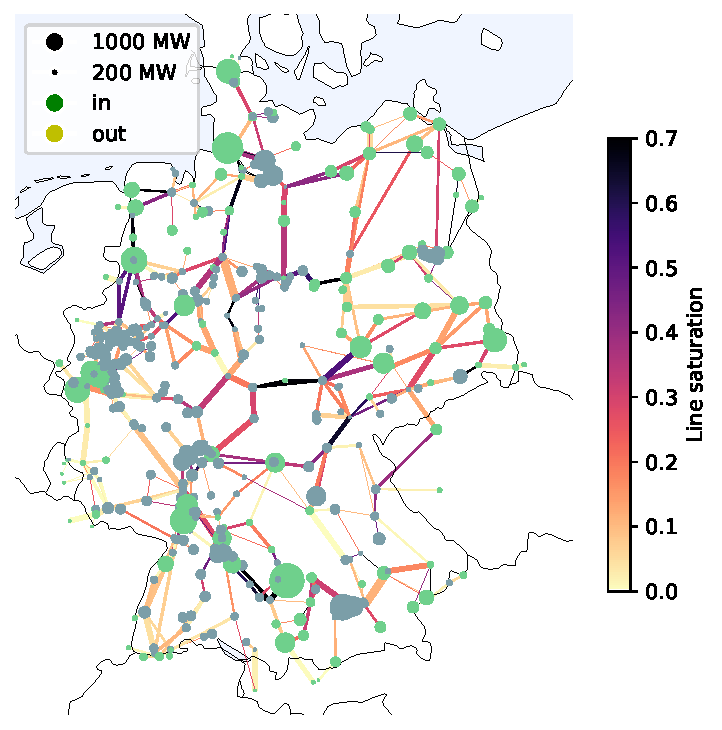
\includegraphics[height=.69\paperheight]{img/nominal_flow_and_injection.pdf}
    \caption{Line saturation at 11am, 1 Jan 2011.}
    \end{figure}
\end{frame}

{
\usebackgroundtemplate{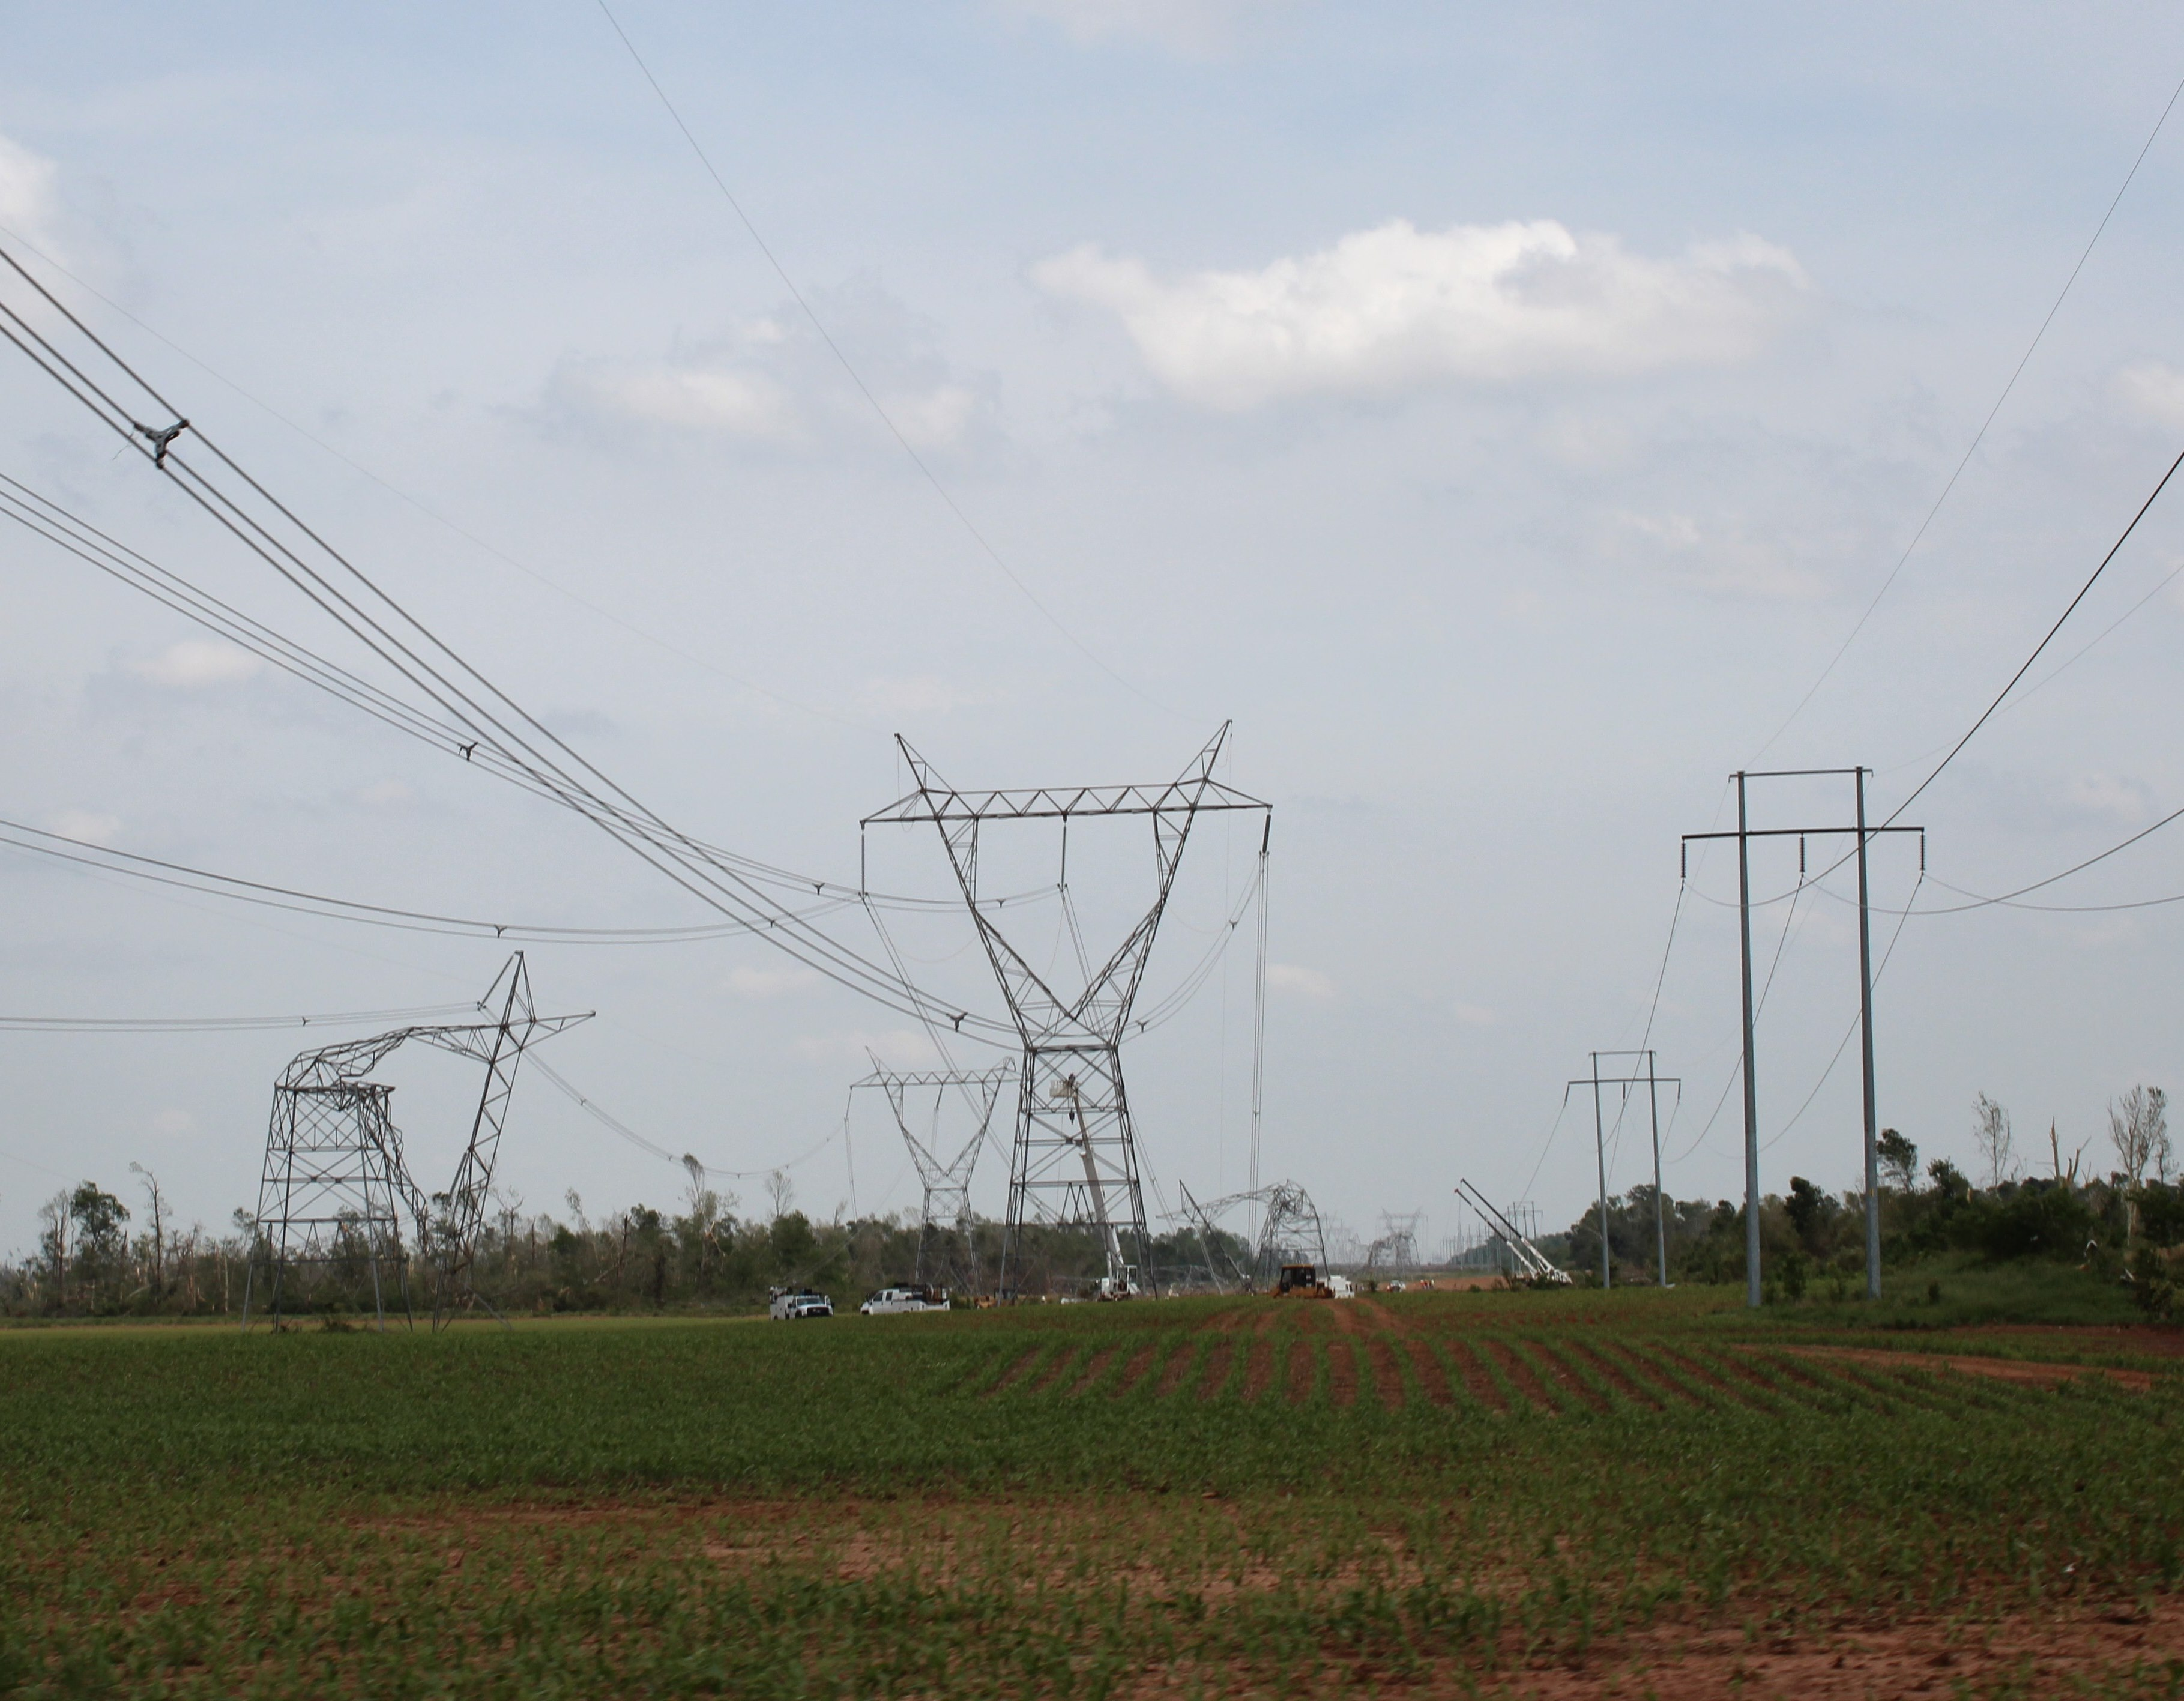
\includegraphics[width=\paperwidth]{img/tornado.jpg}}
\setbeamertemplate{frame footer}{\color{white}{Wikimedia Commons}}
\setbeamertemplate{headline}{\vskip-\headheight}
\begin{frame}[noframenumbering]
\end{frame}

\usebackgroundtemplate{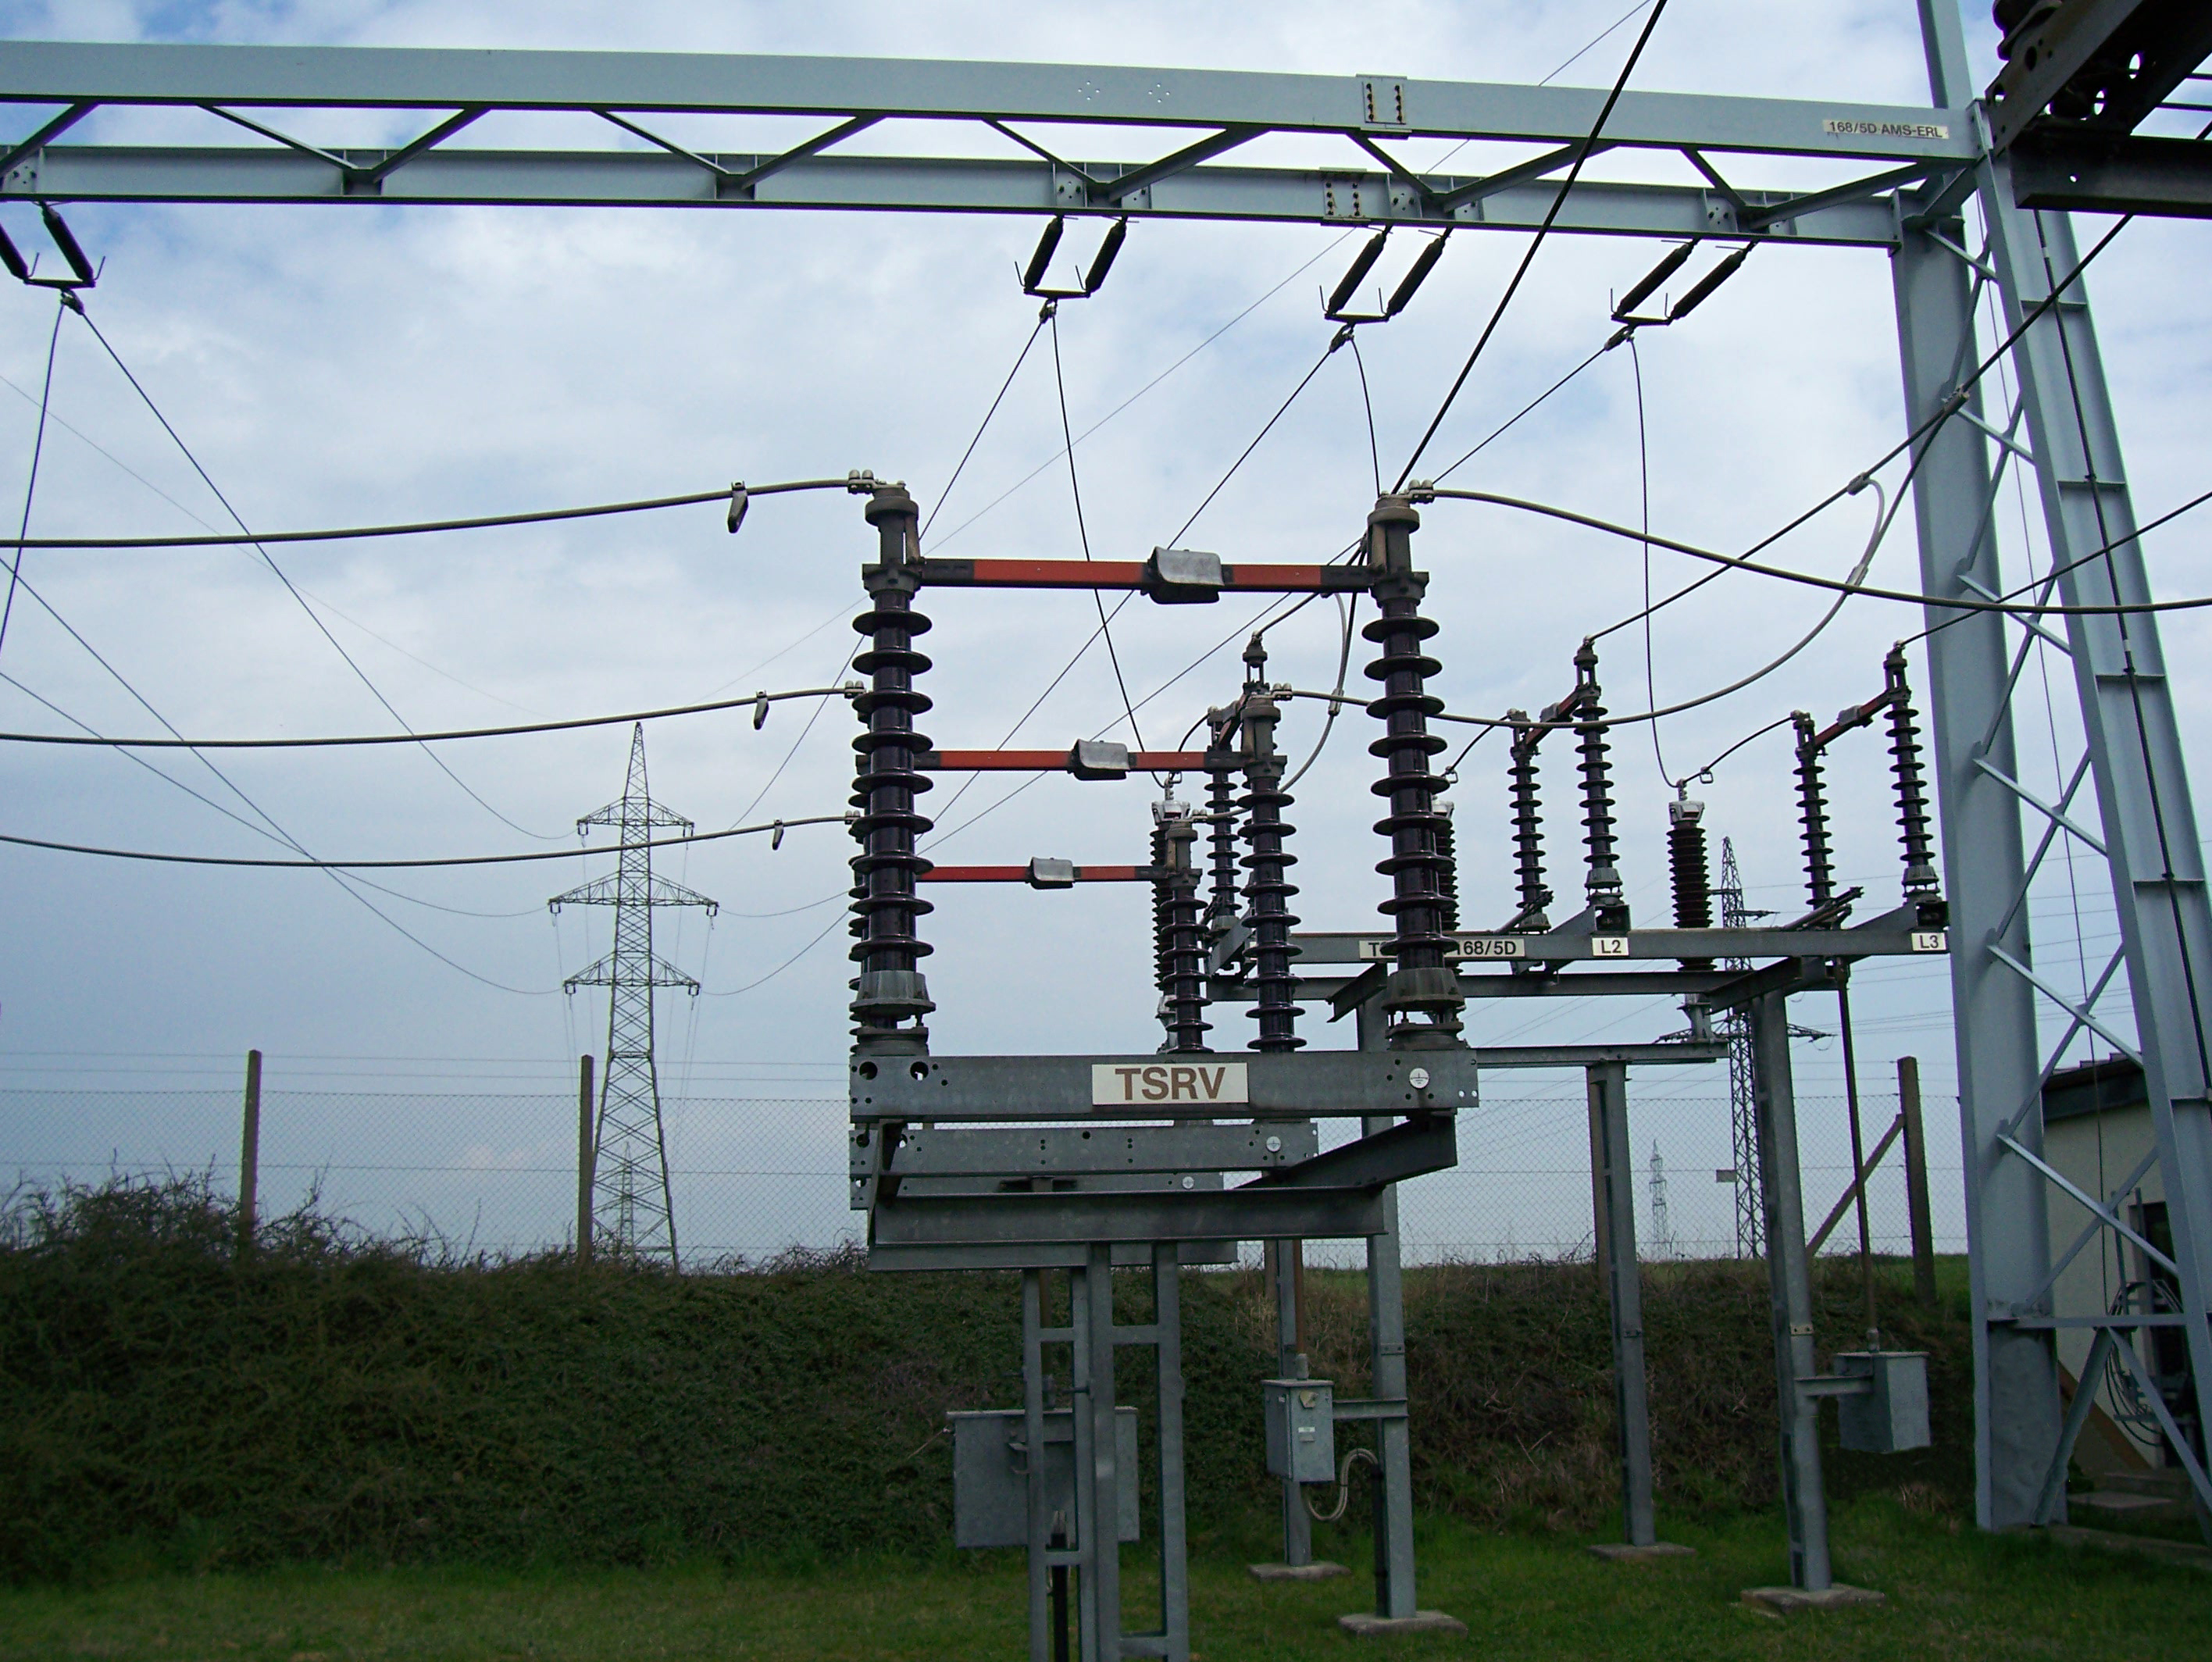
\includegraphics[width=\paperwidth]{img/oostenrijkstoppen.JPG}}
\begin{frame}[noframenumbering]
\end{frame}

\usebackgroundtemplate{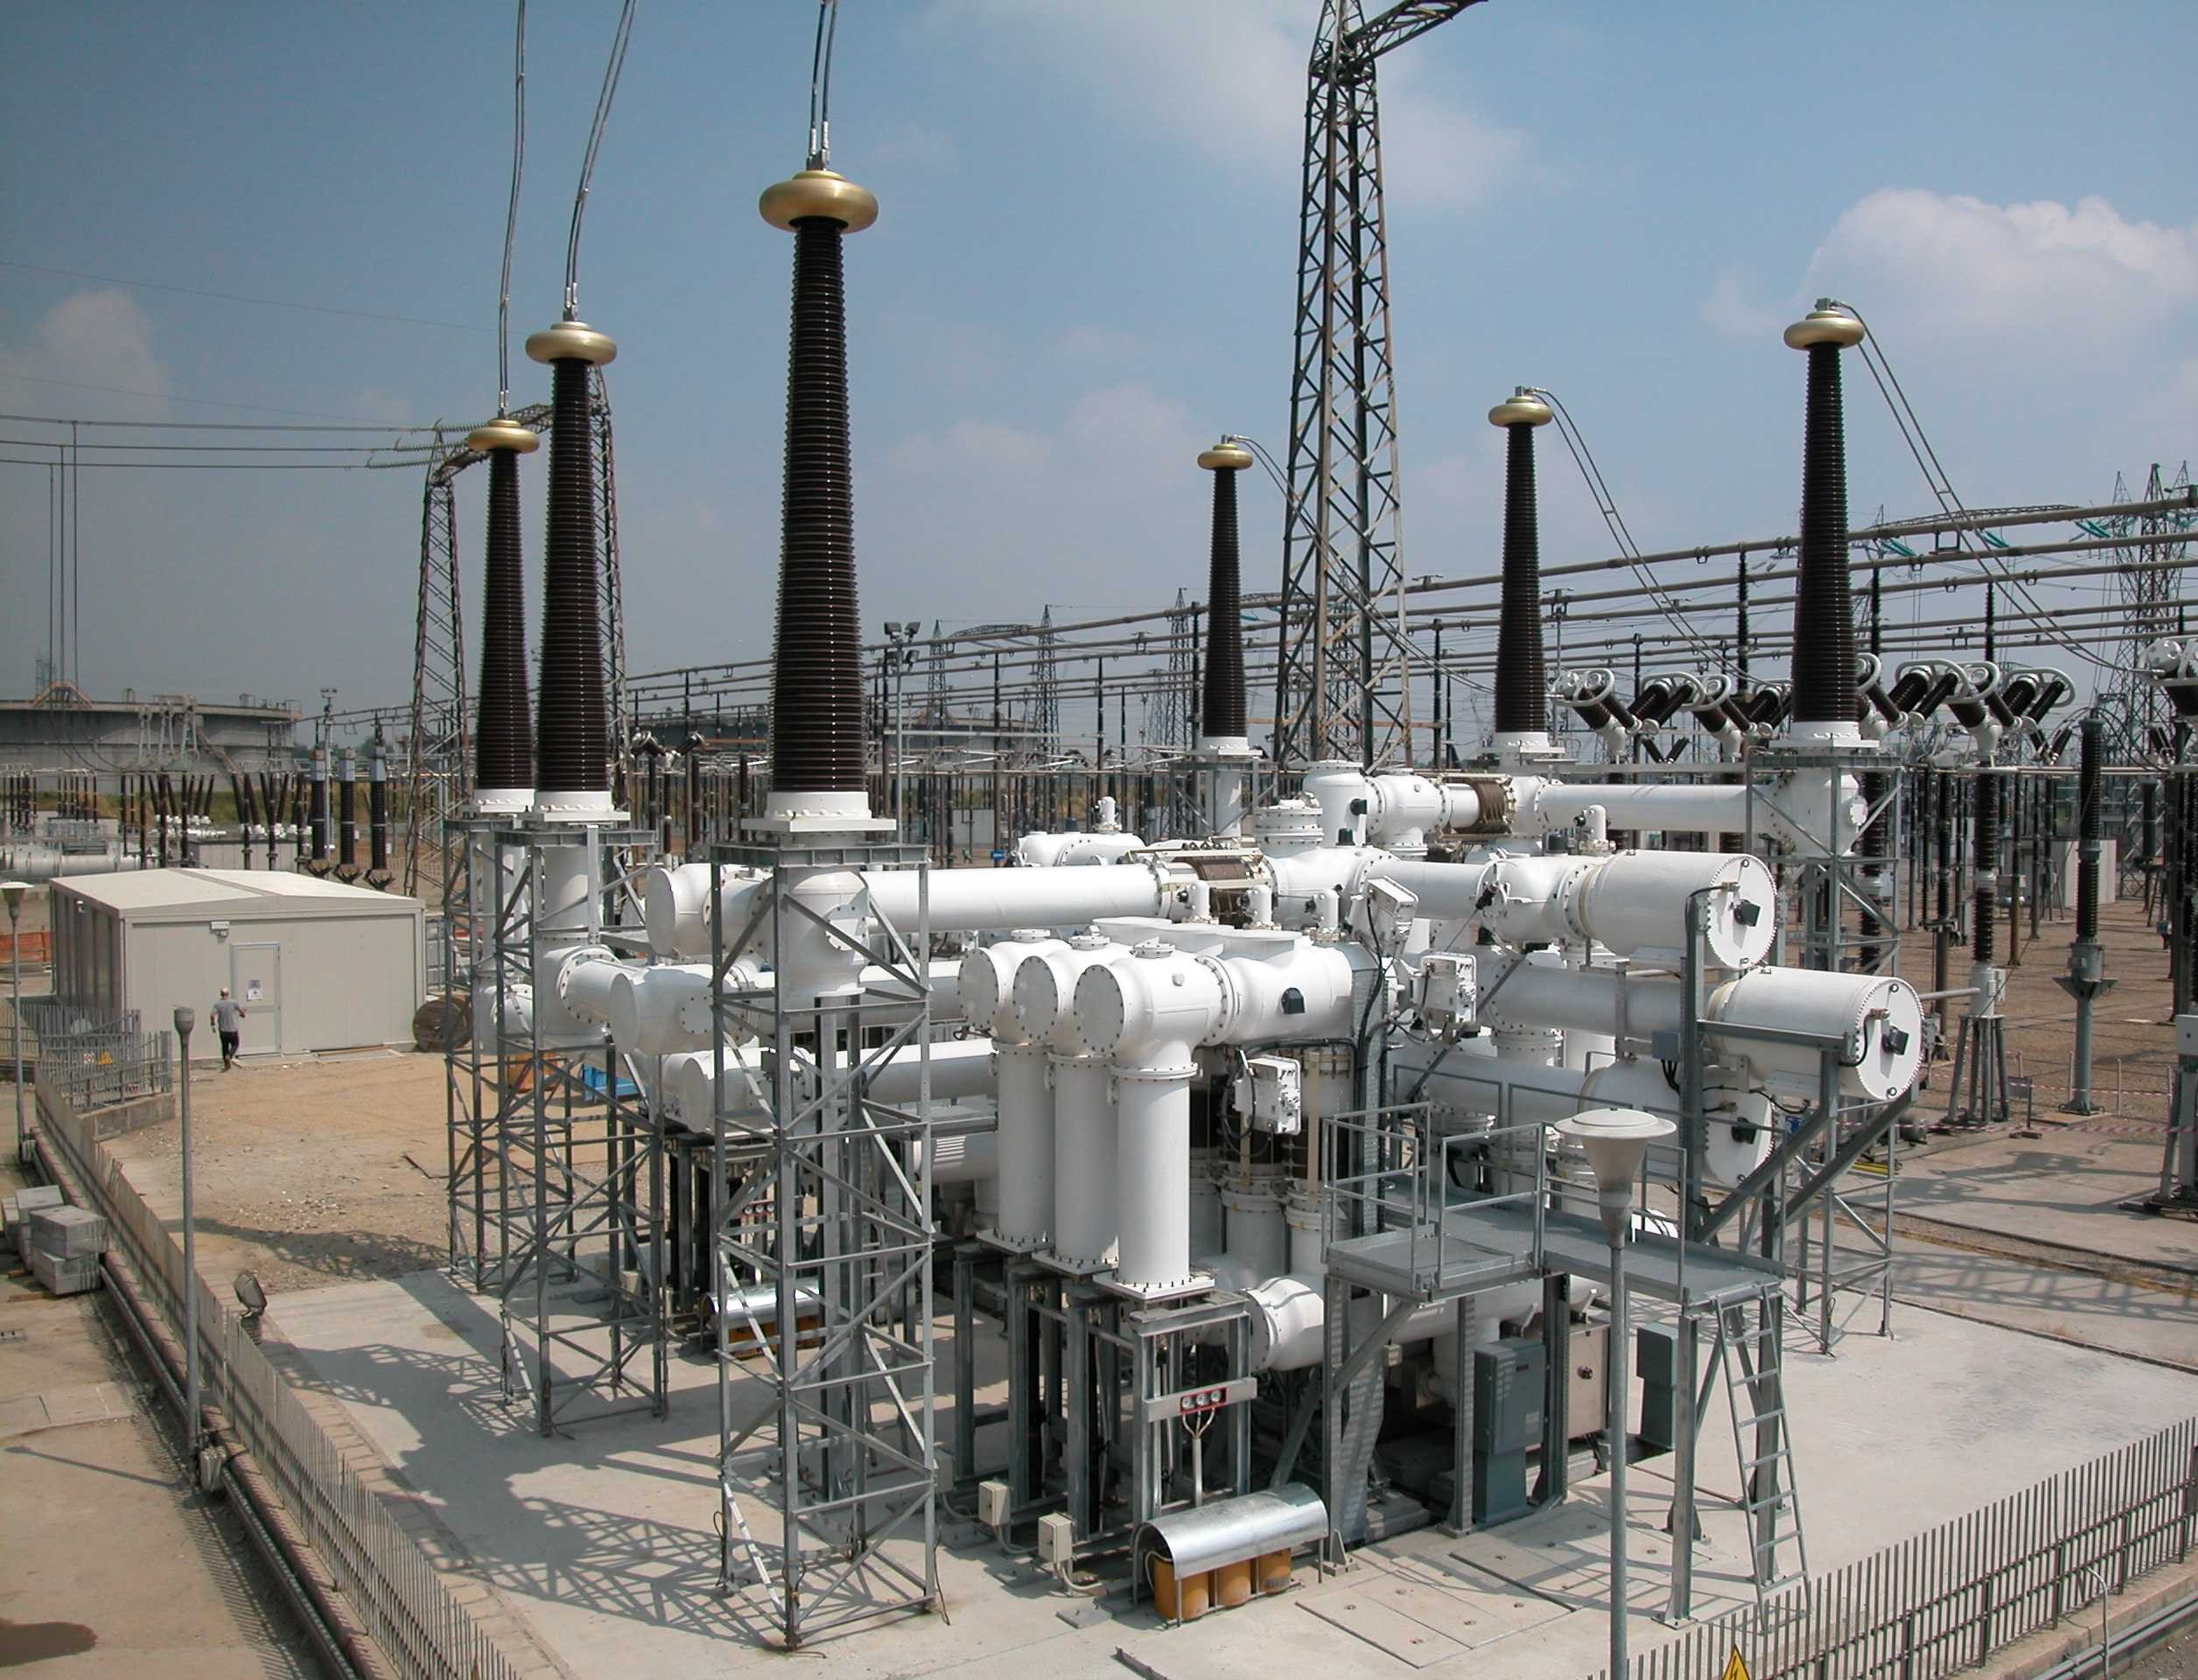
\includegraphics[width=\paperwidth]{img/chinastoppen.jpg}}
\begin{frame}[noframenumbering]
\end{frame}
}

\begin{frame}{Summary}
    \begin{columns}[T,onlytextwidth]
    \column{0.4\textwidth}
    Given:
    \begin{itemize}
        \item Grid structure
        \item Hourly load
        \item Hourly generation
    \end{itemize}
    
    \column{0.6\textwidth}
    Predict:
    \begin{itemize}
        \item \textbf{`Top 10'} of lines most likely to fail
        \item For each risky line: the most likely \textbf{cascading line failures}
    \end{itemize}
    \end{columns}
\end{frame}

{
\usebackgroundtemplate{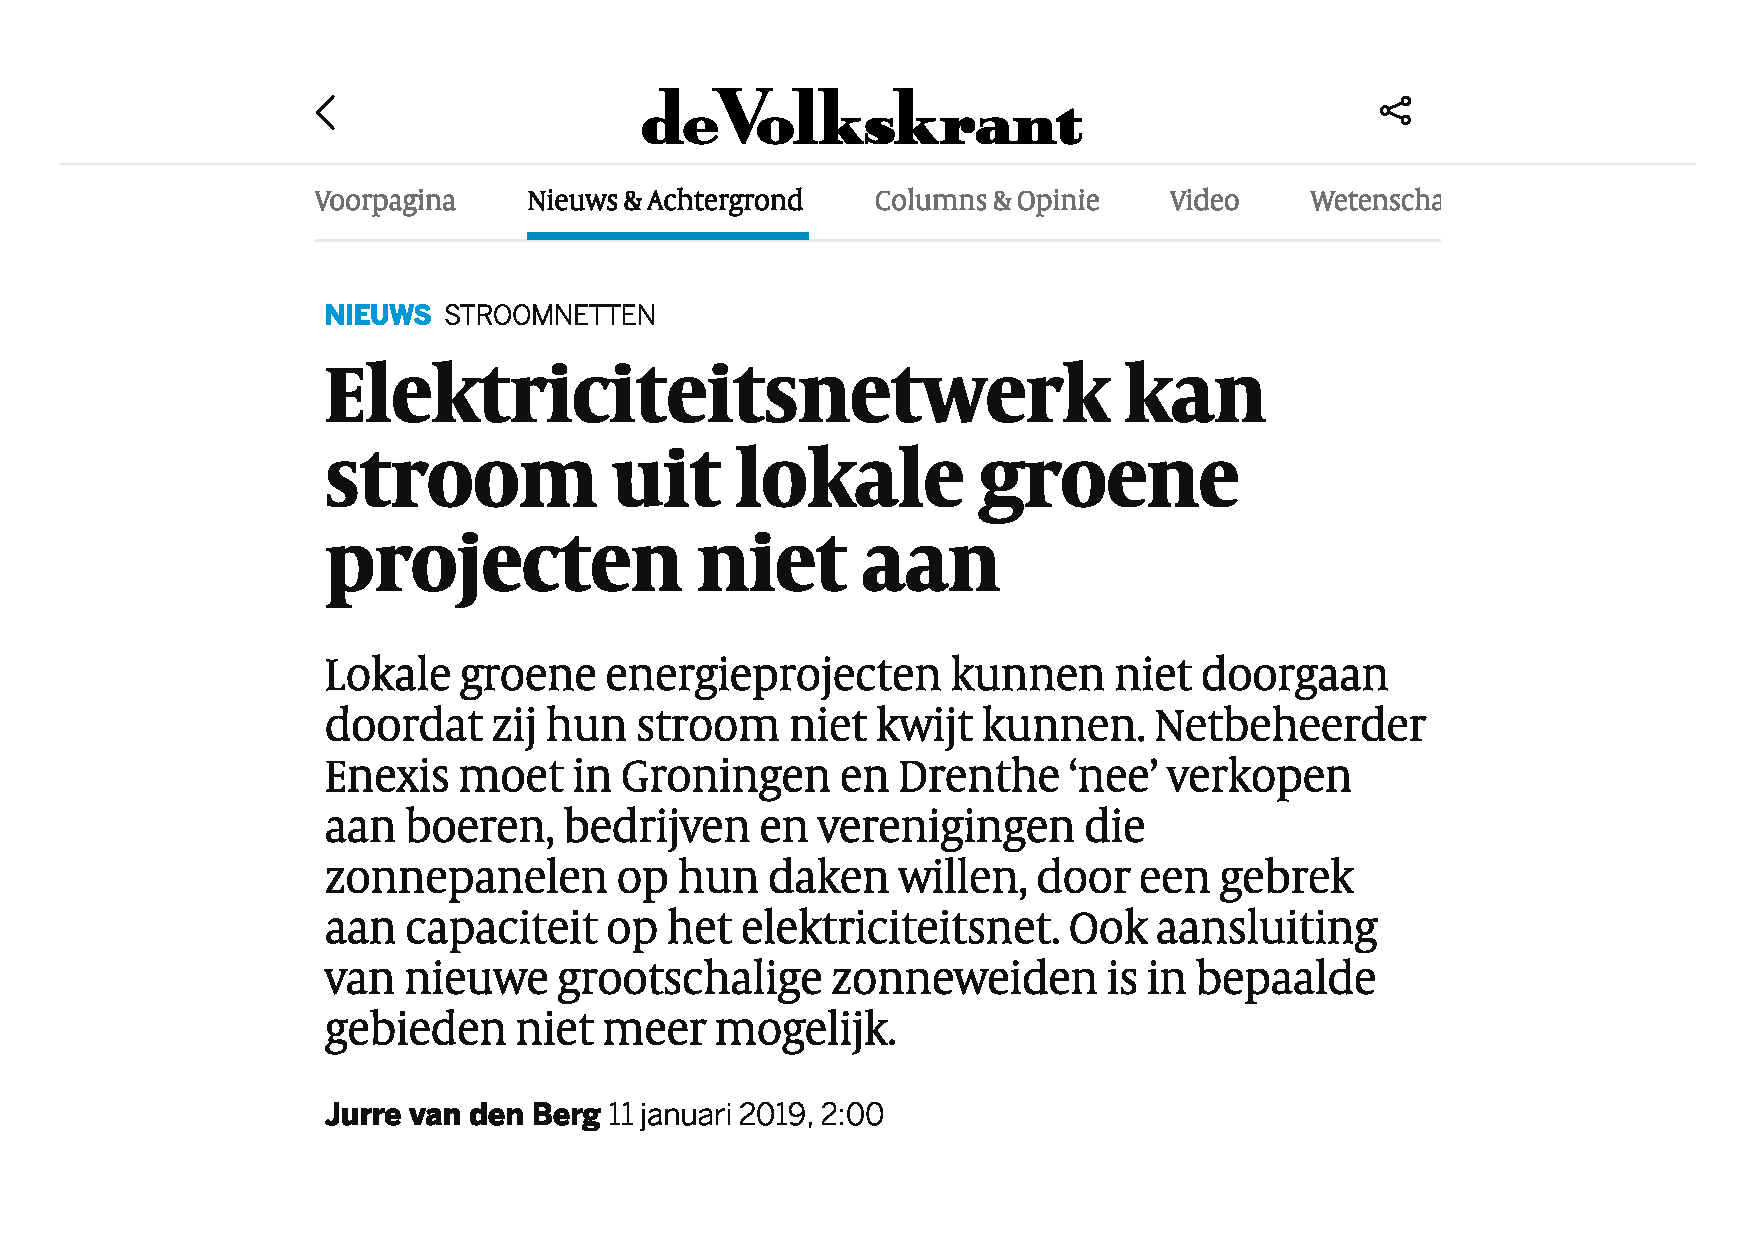
\includegraphics[width=\paperwidth]{img/vk.pdf}}
\begin{frame}[plain]
\end{frame}
}

{
\usebackgroundtemplate{\begin{tikzpicture}{\node[inner sep=0,outer sep=0, opacity=1]{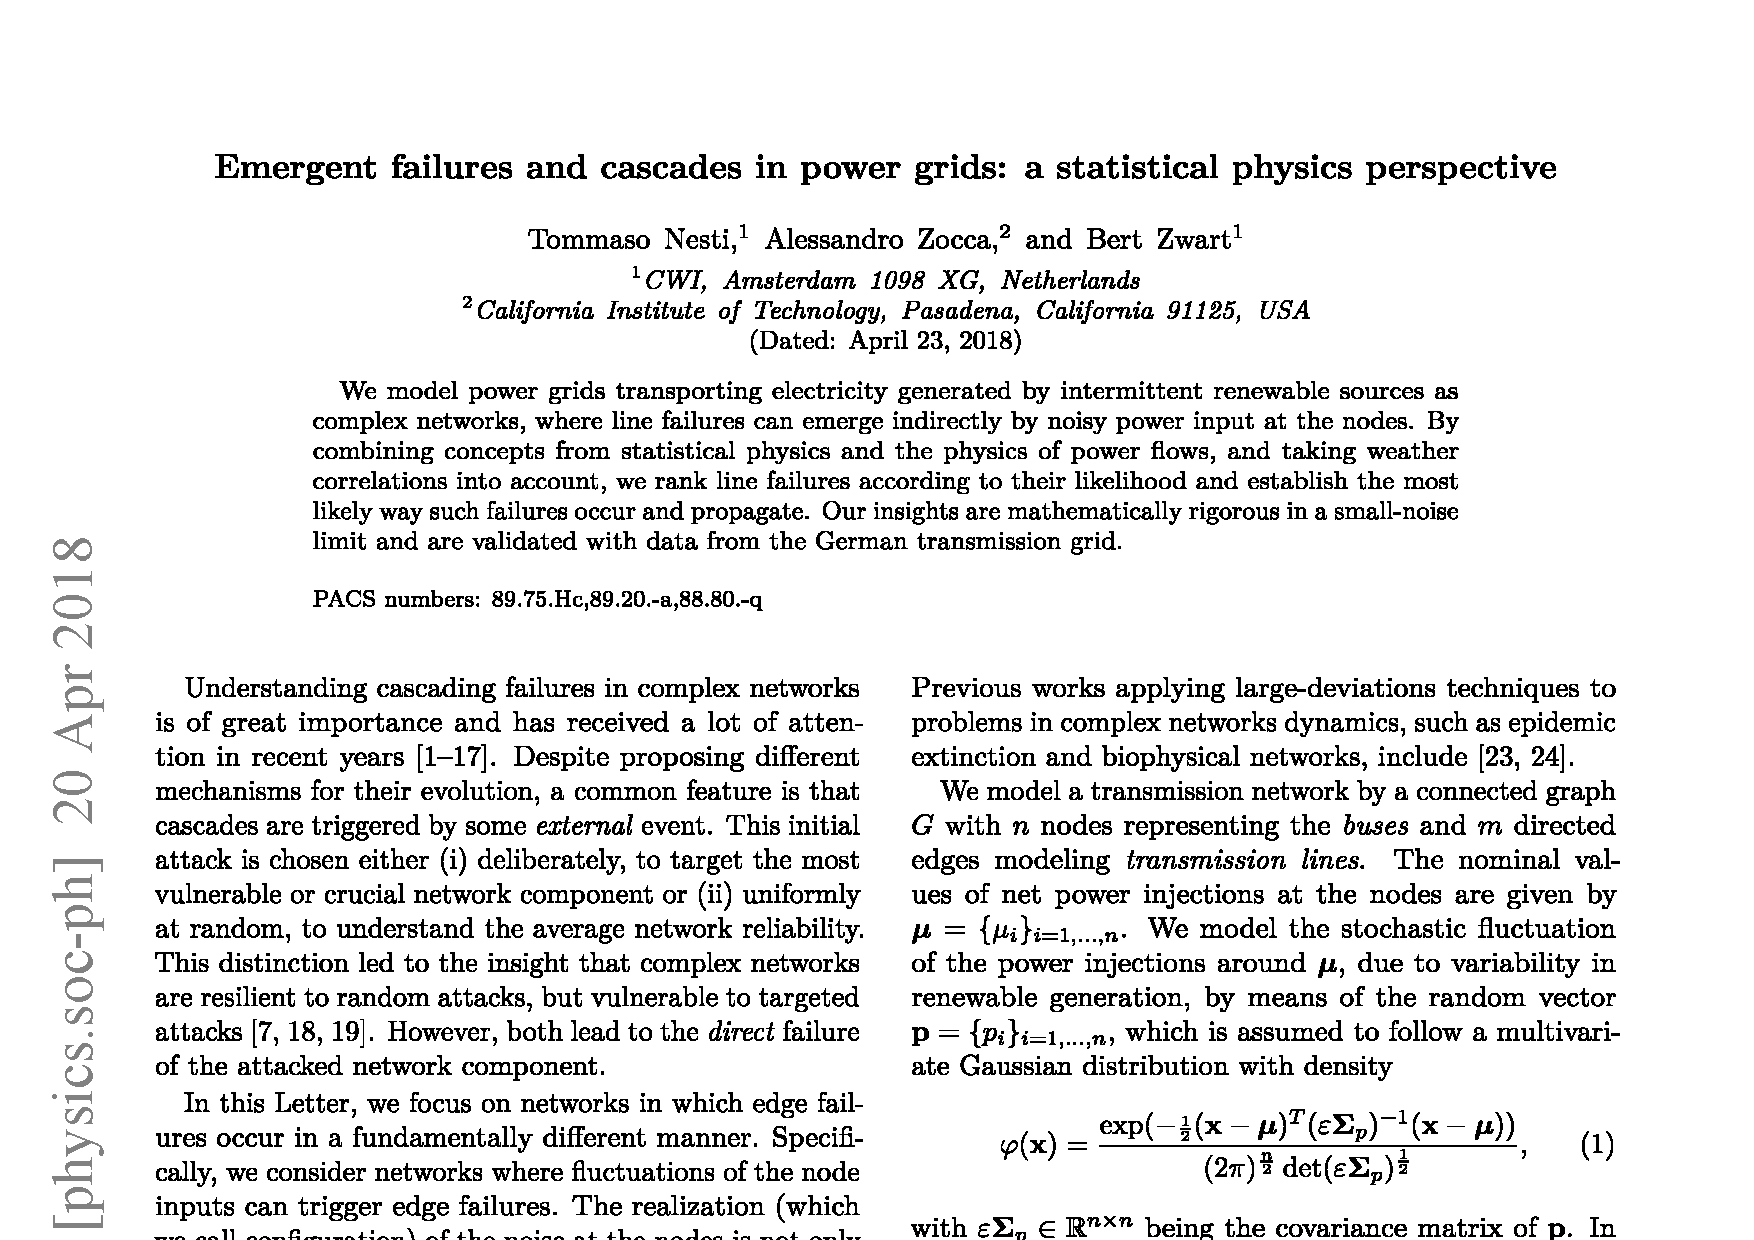
\includegraphics[width=\paperwidth]{img/firstpagenestisnapshot.pdf}};\fill[white,fill opacity=0.01] (0,0) rectangle ($(1cm,5.5cm)$);}\end{tikzpicture}}
\begin{frame}[plain]
\end{frame}
}

\section{Power Flow}

\begin{frame}{Digraph flow}
    \begin{figure}
        \centering
        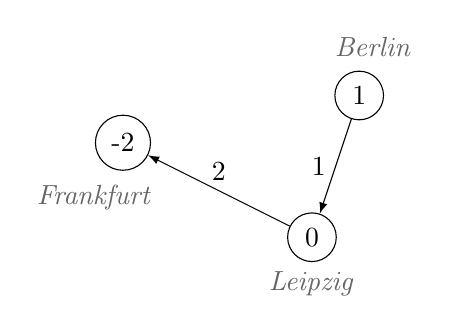
\begin{tikzpicture}[scale=.6]
        \node[draw, circle](b) at (6,3){1};
        \node[draw, circle](f) at (1,2){-2};
        \node[draw, circle](l) at (5,0){0};
        \node[above, opacity=.6] at ($(b.north) + (.3,.1)$) {\emph{Berlin   }};
        \node[below, opacity=.6] at ($(f.south) - (.6,.1)$) {\emph{Frankfurt}};
        \node[below, opacity=.6] at (l.south) {\emph{Leipzig  }};
        
        \draw[-latex] (b) -- node[midway, left] {1} (l);
        \draw[-latex] (l) -- node[midway, above]{2} (f);
        \end{tikzpicture}
    \end{figure}
\end{frame}

\begin{frame}{Puzzle!}
    \begin{figure}
        \centering
        \graafjeduitsland
        {?}
        {?}
        {?}
        {?}
        {1}
        {2}
        {6}
        {-1}
        {4}
    \end{figure}
\end{frame}
\begin{frame}{Solution}
    \begin{figure}
        \centering
        \graafjeduitsland
        {-6}
        {5}
        {0}
        {1}
        {1}
        {2}
        {6}
        {-1}
        {4}
    \end{figure}
\end{frame}
\begin{frame}{Transmission}
    \begin{columns}[T,onlytextwidth]
    \column{0.5\textwidth}
    \[\mat{f}=\begin{pmatrix}
    1\\2\\6\\-1\\4
    \end{pmatrix} \in \mathbb{R}^k, \quad \mat{p}=\begin{pmatrix}
    ?\\?\\?\\?
    \end{pmatrix}\in \mathbb{R}^n\]
    {\metroset{block=fill}
    \begin{block}{\textbf{Power transmission is linear}}
        \[\mat{p} = \mat{C}\cdot \mat{f}\]
      \end{block}
      }
    \[\mat{C} \in \mathbb{R}^{n\times k}\]
    \column{0.5\textwidth}
    \graafjeduitsland
        {?}
        {?}
        {?}
        {?}
        {1}
        {2}
        {6}
        {-1}
        {4}
    \end{columns}
\end{frame}
\begin{frame}{Transmission}
    \begin{columns}[T,onlytextwidth]
    \column{0.5\textwidth}
    {\metroset{block=fill}
    \begin{block}{\textbf{Power transmission is linear}}
        \[\mat{p} = \mat{C}\cdot \mat{f}\]
      \end{block}
      }
    \[\mat{C}=\begin{pmatrix}
    +1& 0&-1&+1& 0\\
     0& 0& 0&-1&+1\\
     0&-1&+1& 0&-1\\
    -1&+1& 0& 0& 0\\
    \end{pmatrix}\]
    \[\text{we get: } \mat{p}=\mat{C}\cdot\mat{f}=\begin{pmatrix}
    -6\\5\\0\\1
    \end{pmatrix}\]
    \column{0.5\textwidth}
    \graafjeduitsland
        {-6}
        {5}
        {0}
        {1}
        {1}
        {2}
        {6}
        {-1}
        {4}
    \end{columns}
\end{frame}

\begin{frame}{Inverse problem: Linear Power Flow (LPF)}
    \begin{figure}
        \centering
        \graafjeduitsland
        {-7}
        {5}
        {1}
        {1}
        {?}
        {?}
        {?}
        {?}
        {?}
    \end{figure}
\end{frame}

\begin{frame}{Solution}
    \begin{figure}
        \centering
        \graafjeduitsland
        {-7}
        {5}
        {1}
        {1}
        {1}
        {2}
        {7}
        {-1}
        {4}
    \end{figure}
\end{frame}

\begin{frame}{Another solution}
    \begin{figure}
        \centering
        \graafjeduitsland
        {-7}
        {5}
        {1}
        {1}
        {0}
        {1}
        {6}
        {-1}
        {4}
    \end{figure}
\end{frame}

\begin{frame}{Inverse problem: Linear Power Flow (LPF)}
    \begin{figure}
        \centering
        \graafjeduitsland
        {-7}
        {5}
        {1}
        {1}
        {?}
        {?}
        {?}
        {?}
        {?}
    \end{figure}
\end{frame}

\begin{frame}{Inverse problem: Linear Power Flow (LPF)}
The $\mat{LPF}$ is a (linear) \emph{right-inverse} of $\mat{C}$:
\[
\mat{C} \cdot \mat{LPF} = \mat{I}.
\]
Many linear maps satisfy this property, but there is only one \emph{right} $\mat{LPF}$ that satisfies \textbf{Kirchoff's Circuit Laws} and \textbf{Ohm's Law}.
\\[3em]
The $\mat{LPF}$ is difficult to compute: requires \emph{Singular Value Decomposition} of a $k \times k$ matrix.
\end{frame}

\begin{frame}{Electric model - HV Layer}
  \begin{figure}
      \centering
      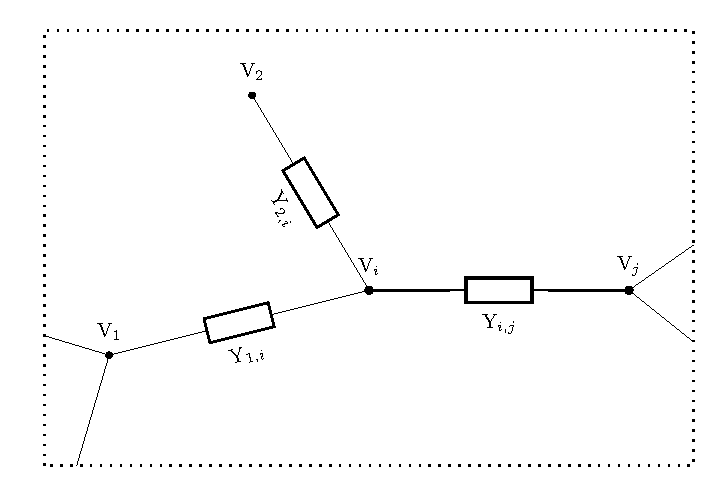
\includegraphics[width=.8\textwidth]{img/vettegraaftoplayer.pdf}
      \caption{Top layer of the electric circuit used in the model. Transmission lines are modelled as impedances.}
      \label{fig:my_label}
  \end{figure}
\end{frame}

{
\usebackgroundtemplate{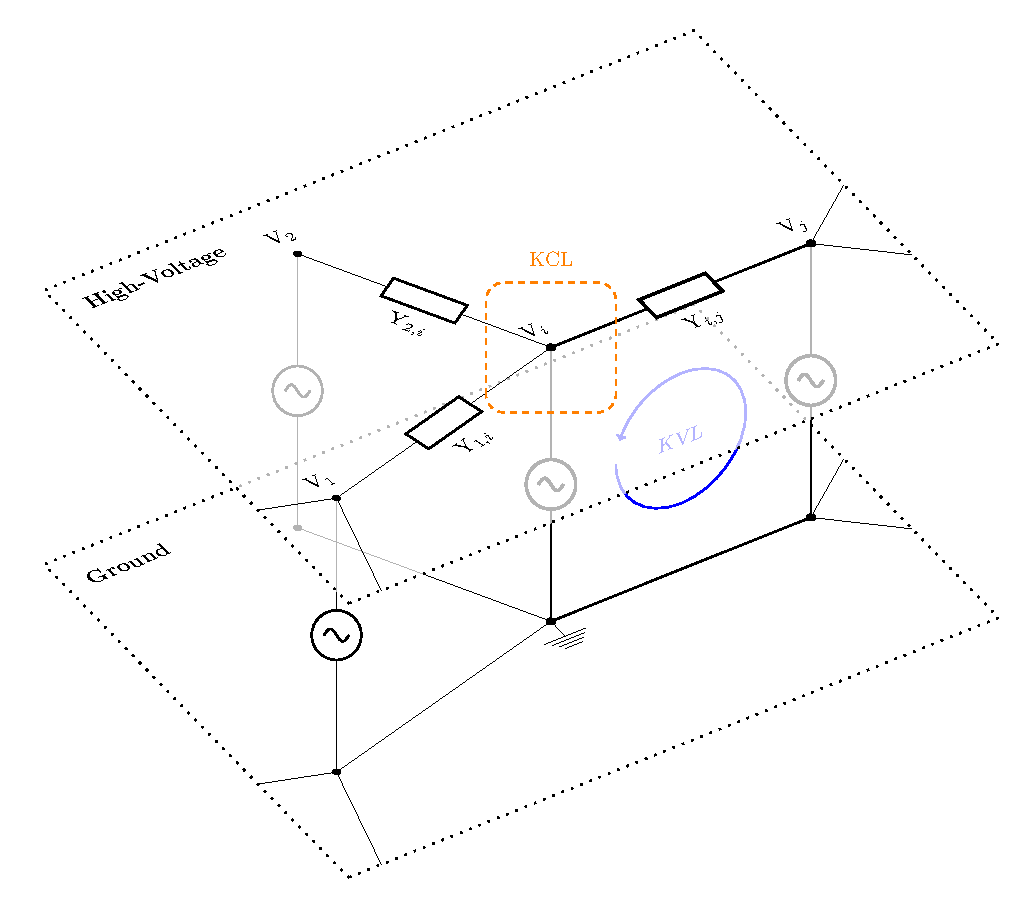
\includegraphics[width=\paperwidth, trim={0 0 0 10mm},clip]{img/vettegraaf.pdf}}
\begin{frame}[plain]
\end{frame}
}

\begin{frame}{Unknown generation: Linear Optimum Power Flow (LOPF)}
    \begin{figure}
        \centering
        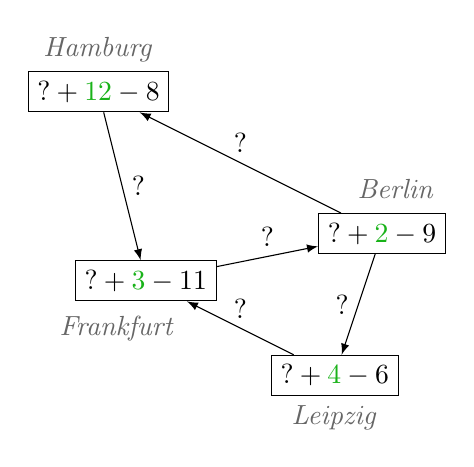
\begin{tikzpicture}[scale=.6]
        \node[draw, rectangle](b) at (6,3){$?+{\color{renewablegreen}{2}}-9$};
        \node[draw, rectangle](h) at (0,6){$?+{\color{renewablegreen}{12}}-8$};
        \node[draw, rectangle](f) at (1,2){$?+{\color{renewablegreen}{3}}-11$};
        \node[draw, rectangle](l) at (5,0){$?+{\color{renewablegreen}{4}}-6$};
        \node[above, opacity=.6] at ($(b.north) + (.3,.1)$) {\emph{Berlin   }};
        \node[above, opacity=.6] at (h.north) {\emph{Hamburg  }};
        \node[below, opacity=.6] at ($(f.south) - (.6,.1)$) {\emph{Frankfurt}};
        \node[below, opacity=.6] at (l.south) {\emph{Leipzig  }};
        
        \draw[-latex] (b) -- node[midway, left] {?} (l);
        \draw[-latex] (l) -- node[midway, above]{?} (f);
        \draw[-latex] (f) -- node[midway, above]{?} (b);
        \draw[-latex] (b) -- node[midway, above]{?} (h);
        \draw[-latex] (h) -- node[midway, right]{?} (f);
\end{tikzpicture}
    \end{figure}
\end{frame}

\begin{frame}{Unknown generation: Optimum Power Flow (OPF)}
    \begin{figure}
        \centering
        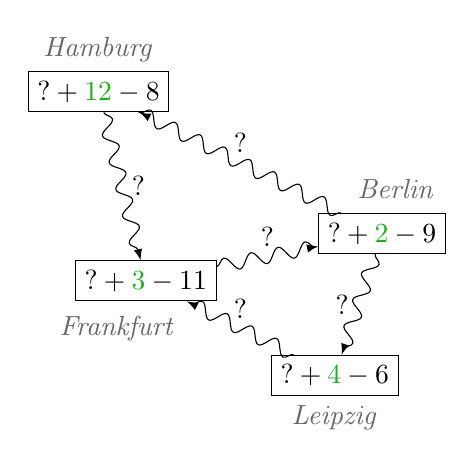
\begin{tikzpicture}[scale=.6, decoration=snake]
    \node[draw, rectangle](b) at (6,3){$?+{\color{renewablegreen}{2}}-9$};
    \node[draw, rectangle](h) at (0,6){$?+{\color{renewablegreen}{12}}-8$};
    \node[draw, rectangle](f) at (1,2){$?+{\color{renewablegreen}{3}}-11$};
    \node[draw, rectangle](l) at (5,0){$?+{\color{renewablegreen}{4}}-6$};
    \node[above, opacity=.6] at ($(b.north) + (.3,.1)$) {\emph{Berlin   }};
    \node[above, opacity=.6] at (h.north) {\emph{Hamburg  }};
    \node[below, opacity=.6] at ($(f.south) - (.6,.1)$) {\emph{Frankfurt}};
    \node[below, opacity=.6] at (l.south) {\emph{Leipzig  }};
    
    \draw[-latex, decorate] (b) -- node[midway, left] {?} (l);
    \draw[-latex, decorate] (l) -- node[midway, above]{?} (f);
    \draw[-latex, decorate] (f) -- node[midway, above]{?} (b);
    \draw[-latex, decorate] (b) -- node[midway, above]{?} (h);
    \draw[-latex, decorate] (h) -- node[midway, right]{?} (f);
\end{tikzpicture}
    \end{figure}
\end{frame}


{
\usebackgroundtemplate{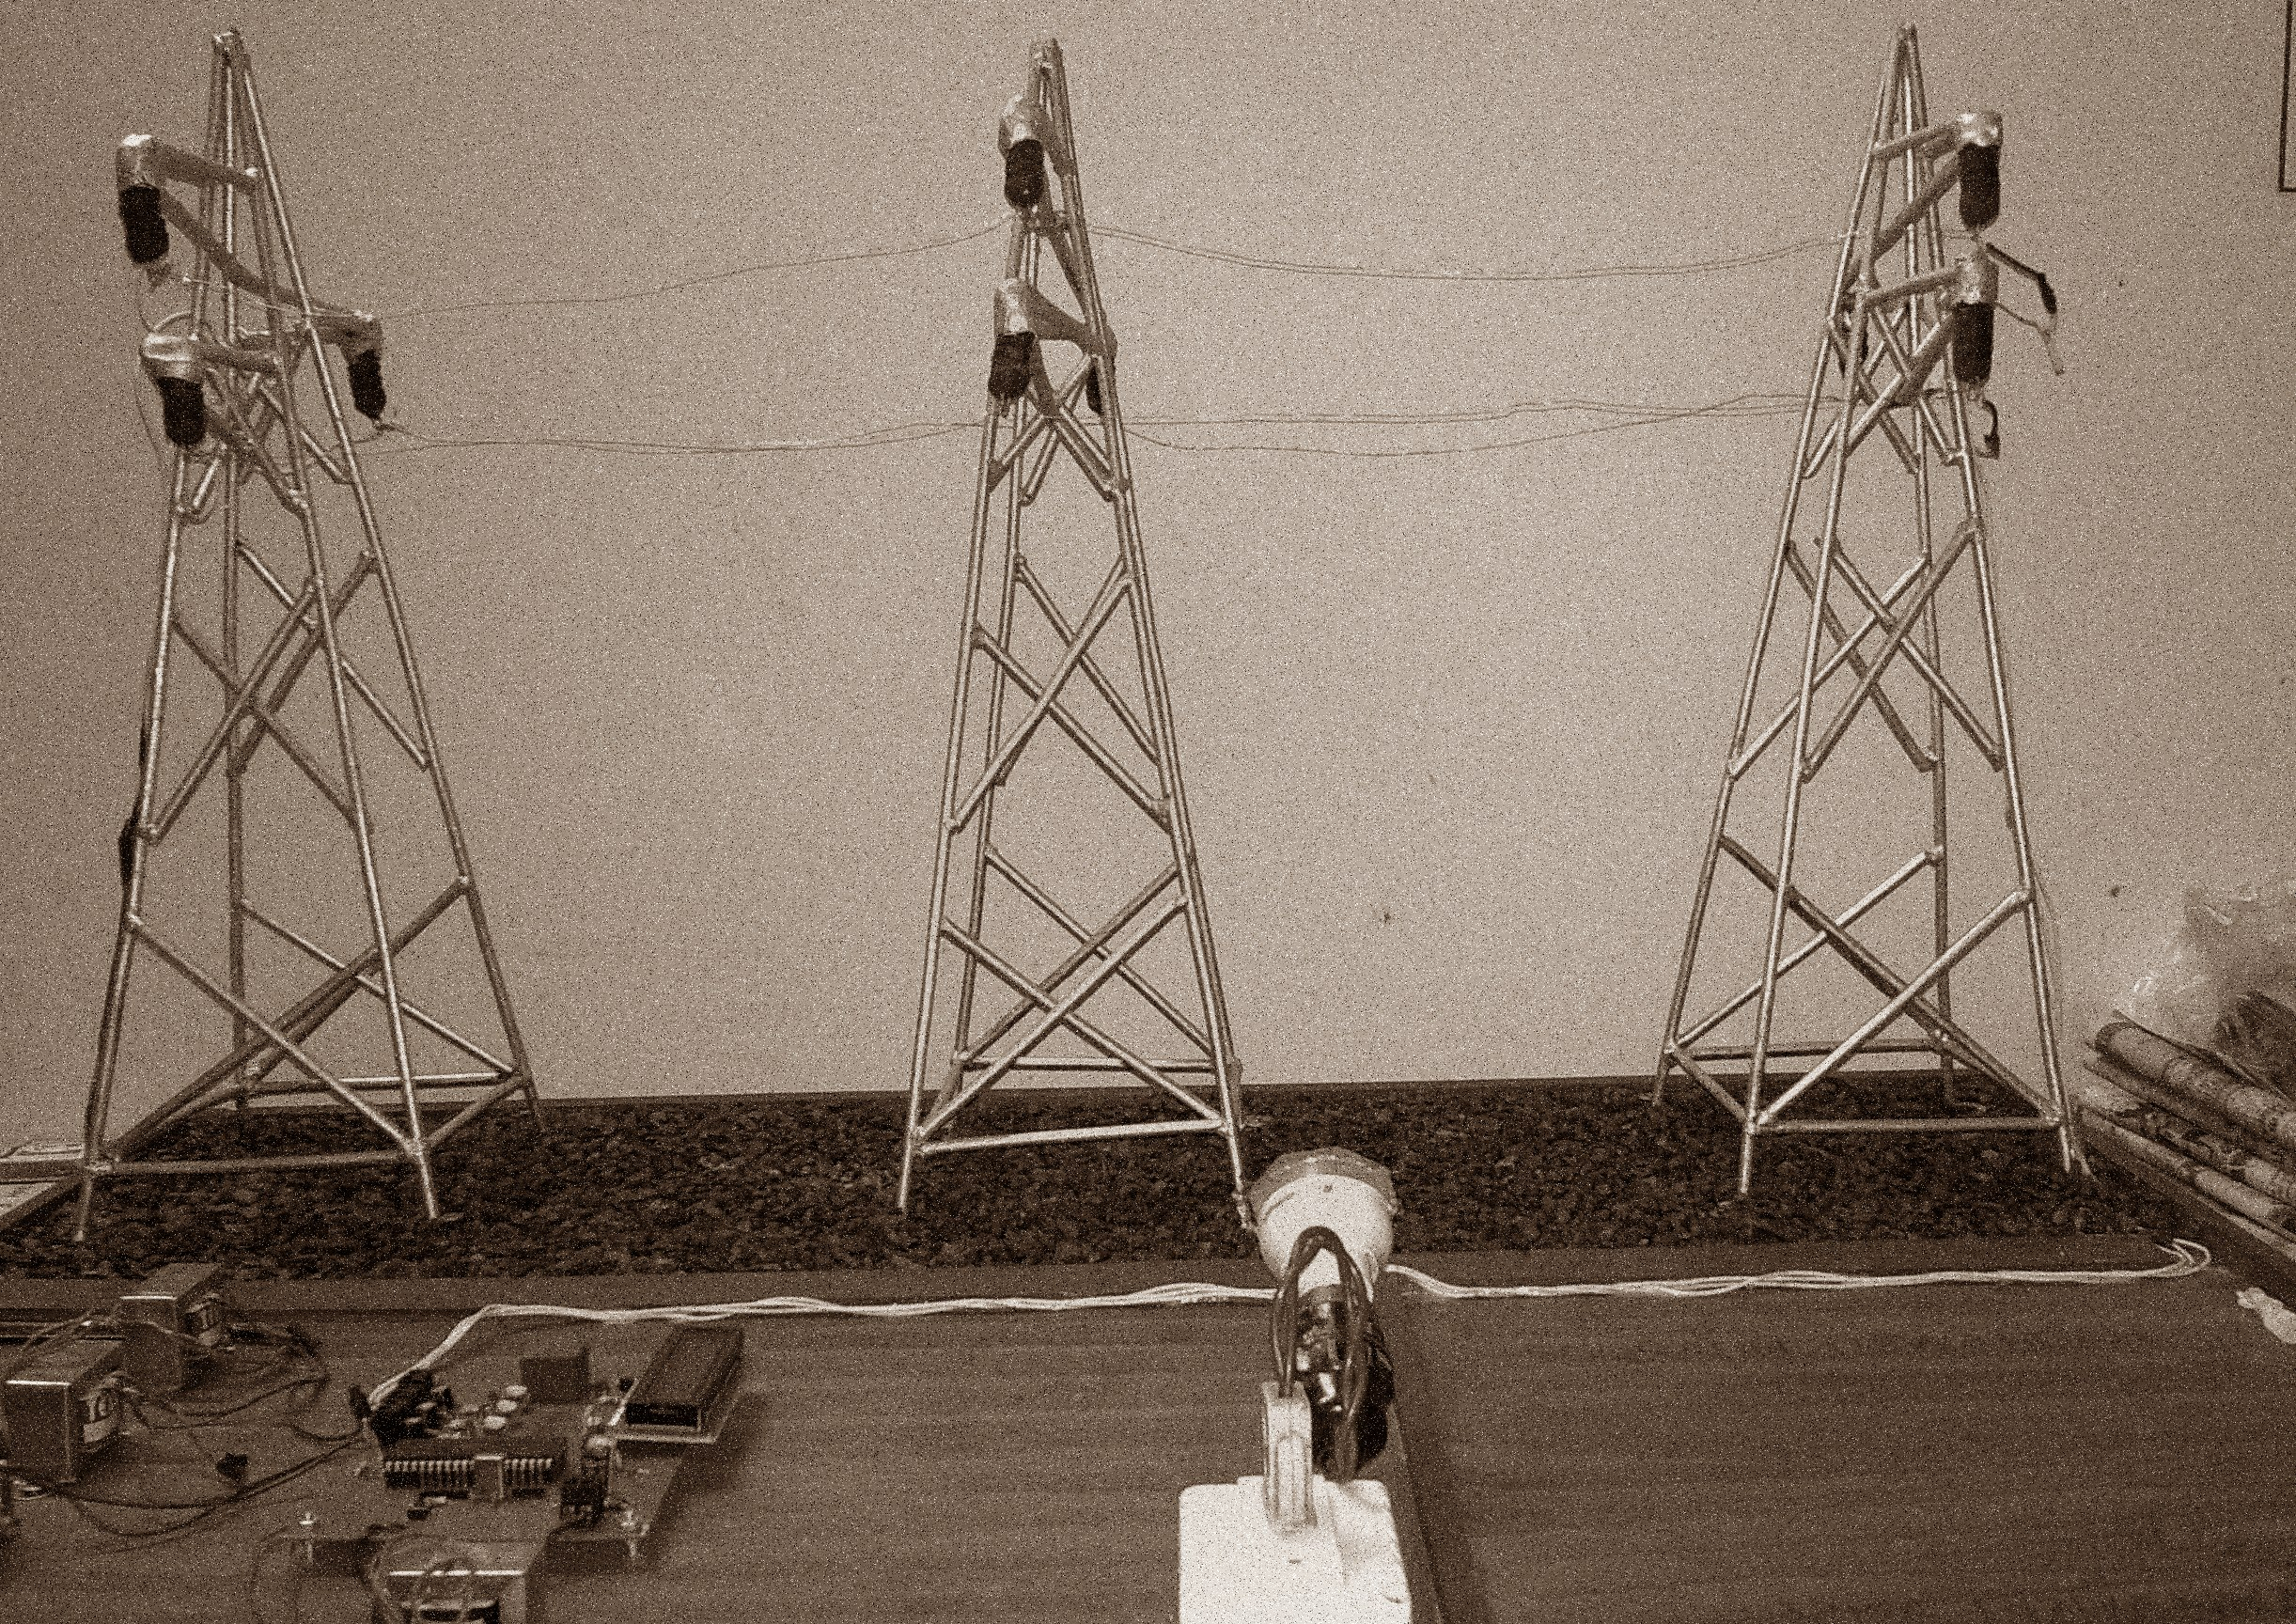
\includegraphics[height=\paperheight]{img/schaalmodel_sepia.jpg}}
\setbeamertemplate{frame footer}{\color{white}{Instructables	}}
\setbeamertemplate{headline}{\vskip-\headheight}
\begin{frame}[noframenumbering]

\end{frame}
}


\begin{frame}{OPF to supplement data}
\begin{columns}[T,onlytextwidth]
    \column{0.4\textwidth}
    Available:
    \begin{itemize}
        \item Grid structure
        \item Hourly load
        \item Hourly \alert{solar and wind} generation
    \end{itemize}
    Not available:
    \begin{itemize}
        \item Hourly \alert{grey} generation
    \end{itemize}
    
    \column{0.2\textwidth}
    \vspace{20mm}
    \[\tikz{\draw[->,thick] (0,0) -- (15mm,0) node[above,midway] {OPF};}\]
    \column{0.4\textwidth}
    Available:
    \begin{itemize}
        \item Grid structure
        \item Hourly load
        \item Hourly generation
    \end{itemize}
    \end{columns}
\end{frame}

\begin{frame}{OPF accuracy}
    OPF is used to generate an \alert{hourly power injection dataset}, by assuming that the cheapest generation profile is used at all times.
    \vspace{10mm}
    {\metroset{block=fill}
    \begin{block}{OPF is a fair approximation, because}
        \emph{grid operators actually use OPF algorithms to minimise costs}
      \end{block}
      }
\end{frame}

\section{Stochastic power injections}

\begin{frame}{Deterministic power injection $\mat{p}$}
    Given a power injection $\mat{p} \in \mathbb{R}^n$:
    \begin{itemize}
        \item \alert{\textbf{Linearised Power Flow} computes \emph{line current}}
        \item $>100\%$ saturated $\Rightarrow$ \textbf{line failure}
    \end{itemize}
    \vspace{10mm}
\[
\begin{pmatrix}
p_1\\
p_2\\
p_3\\
p_4
\end{pmatrix}
\quad
\tikz{\draw[|->,thick] (0,0) -- (10mm,0) node[above,midway] {LPF};}
\quad
\begin{pmatrix}
f_1 = \raisebox{-1mm}{\inlinebar{.5}{green}} \\
f_2 = \raisebox{-1mm}{\inlinebar{.2}{green}} \\
f_3 = \raisebox{-1mm}{\inlinebar{.8}{green}} \\
f_4 = \raisebox{-1mm}{\inlinebar{1.15}{red}} \\
f_5 = \raisebox{-1mm}{\inlinebar{.3}{green}}
\end{pmatrix}
\quad
\tikz{\draw[|->,thick] (0,0) -- (20mm,0) node[above,midway] {$\leq$ threshold};}
\quad
\begin{pmatrix}
\Checkmark\\
\Checkmark\\
\Checkmark\\
\TikzCross\\
\Checkmark
\end{pmatrix}
\]
\end{frame}


\begin{frame}{Stochastic power injection $\mat{P}$}
    When the power injection $\mat{P}$ is \textbf{stochastic}:
    \begin{itemize}
        \item \alert{\textbf{LPF} now gives the line current \emph{distribution}}
        \item For each line, we have:
        \begin{itemize}
            \item the failure \emph{probability}
            \item the \emph{most likely power injection $\tilde{\mat{p}}$} that would cause that failure
        \end{itemize}
    \end{itemize}
    \vspace{10mm}
\[
\hspace{-7mm}
\begin{pmatrix}
P_1\\
P_2\\
P_3\\
P_4
\end{pmatrix}
%
\tikz{\draw[|->,thick] (0,0) -- (10mm,0) node[above,midway] {LPF};}
%
\begin{pmatrix}
F_1 \sim \raisebox{-1mm}{\inlineprob{0.5}{10.0}{orange}} \\
F_2 \sim \raisebox{-1mm}{\inlineprob{0.25}{20.0}{orange}} \\
F_3 \sim \raisebox{-1mm}{\inlineprob{0.9}{100.0}{orange}} \\
F_4 \sim \raisebox{-1mm}{\inlineprob{1.1}{10.0}{orange}} \\
F_5 \sim \raisebox{-1mm}{\inlineprob{0.7}{5.0}{orange}}
\end{pmatrix}
\tikz{\draw[|->,thick] (0,0) -- (10mm,0) node[above,midway] {};}
\begin{pmatrix}
\phantom{0}0.001\%\phantom{0}\\
\phantom{0}0.0001\%\\
\phantom{0}0.1\%\phantom{000}\\
60.0\%\phantom{000}\\
10.0\%\phantom{000}
\end{pmatrix}, 
\begin{pmatrix}
\tilde{\mat{p}}\,\mid \, F_1>1\\
\tilde{\mat{p}}\,\mid \, F_2>1\\
\tilde{\mat{p}}\,\mid \, F_3>1\\
\tilde{\mat{p}}\,\mid \, F_4>1\\
\tilde{\mat{p}}\,\mid \, F_5>1
\end{pmatrix}
\]
\end{frame}

\plaatjeframe

\begin{frame}{Stochastic power injection $\mat{P}$}
When the power injection $\mat{P}$ is \textbf{Gaussian}:
\[
\mat{P} \, \sim \, \mathcal{N}(\mat{\mu}, \Sigma),
\]
then then line flow vector $\mat{F}$ is also Gaussian:
\begin{align*}
\mat{F} &= \mat{LPF}\cdot\mat{P} \\ 
\mat{F} &\sim \, \mathcal{N}(\mat{LPF}\cdot\mat{\mu}, \quad\mat{LPF} \cdot \Sigma \cdot \mat{LPF}^T).
\end{align*}
\end{frame}

\begin{frame}{Correlated injections, night-time}
    \begin{figure}
    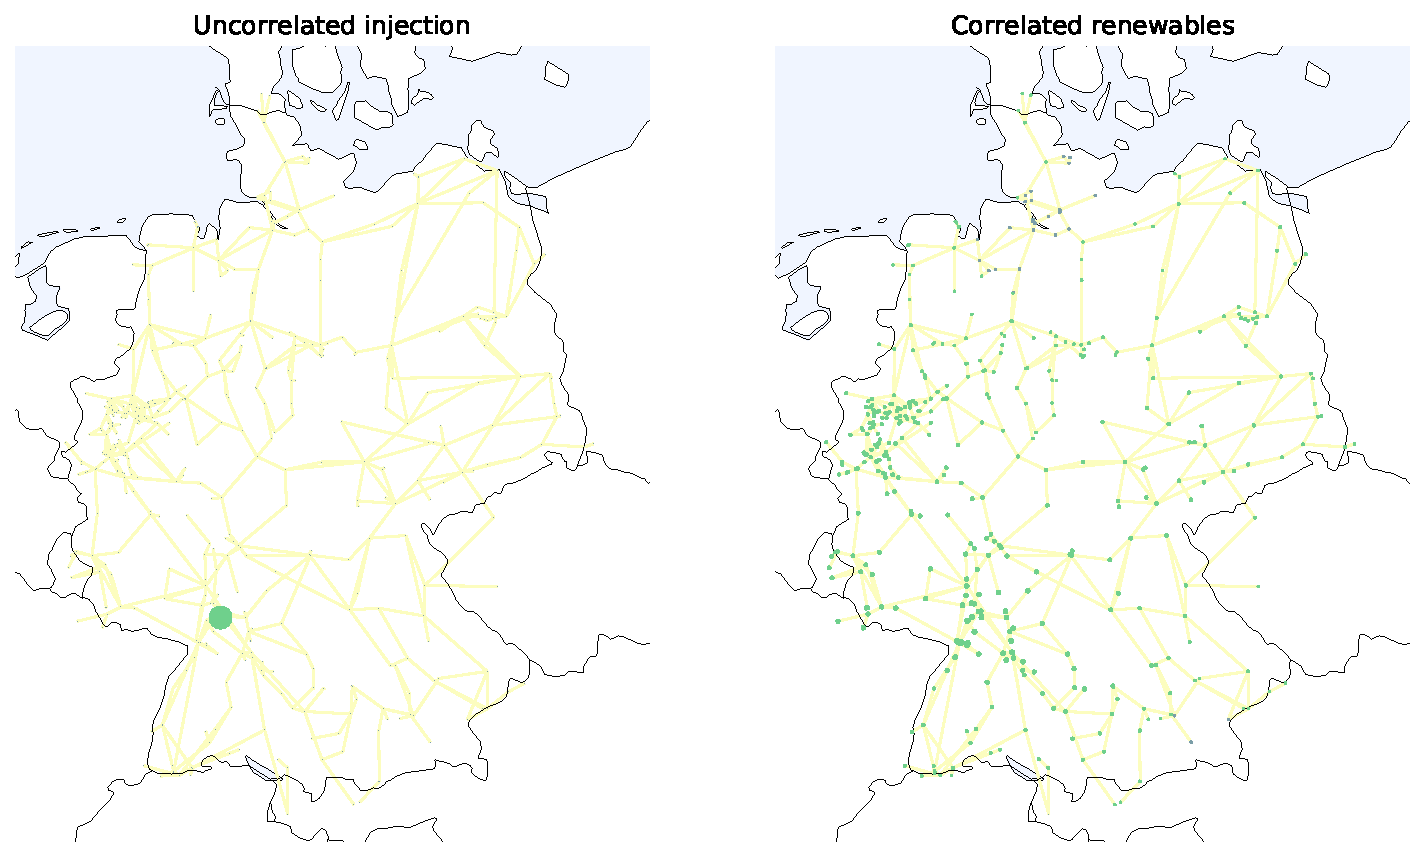
\includegraphics[height=.65\paperheight]{img/bus_correlation_345_iid_and_fullcov_night.pdf}
    \caption{Covariance relative to bus 345, wind only.}
    \end{figure}
\end{frame}

\begin{frame}{Correlated injections, daytime}
    \begin{figure}
    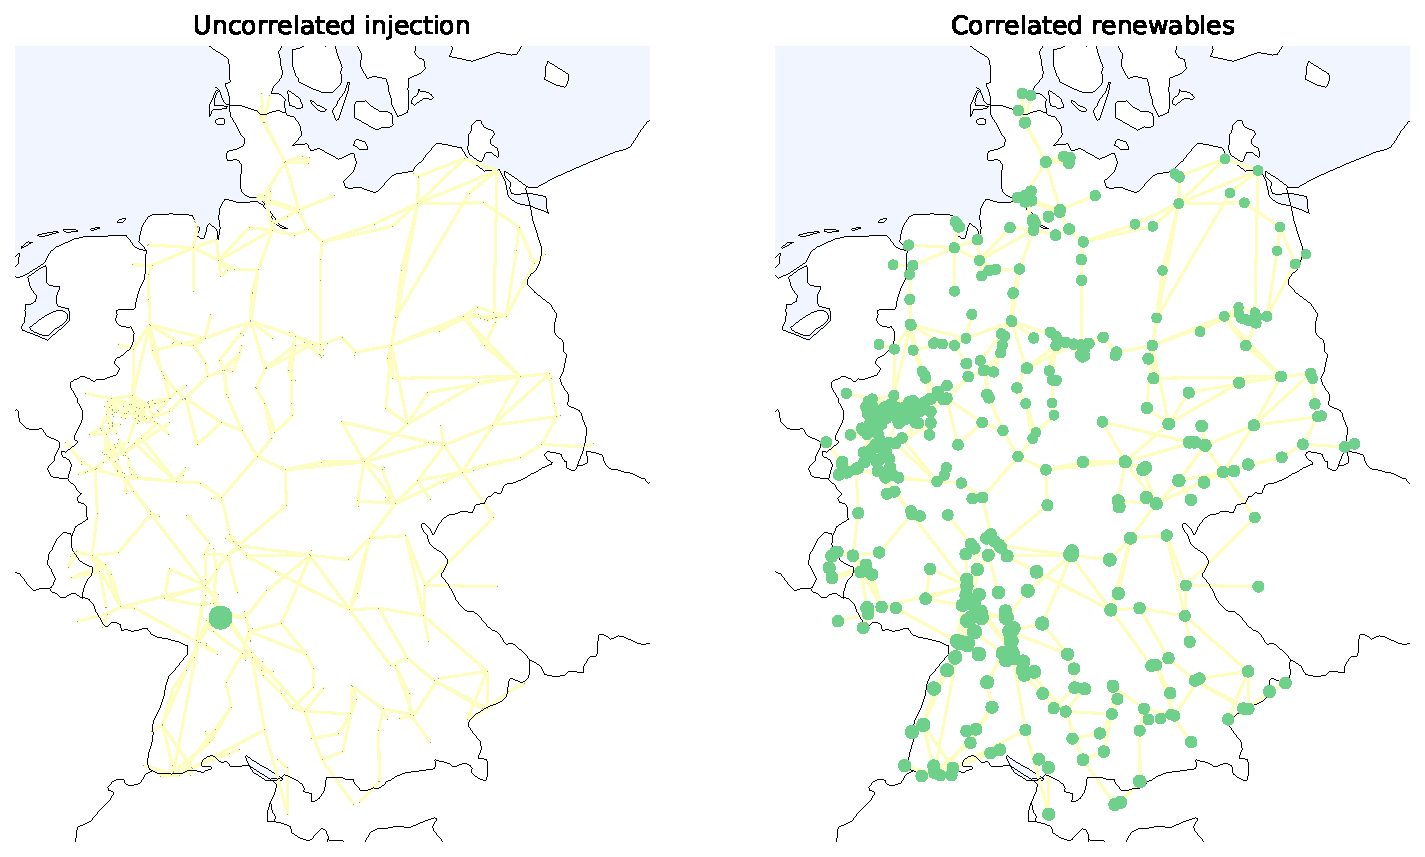
\includegraphics[height=.65\paperheight]{img/bus_correlation_345_iid_and_fullcov_day.pdf}
    \caption{Covariance relative to bus 345, wind \& solar.}
    \end{figure}
\end{frame}

\begin{frame}{Correlated flow, daytime}
    \begin{figure}
    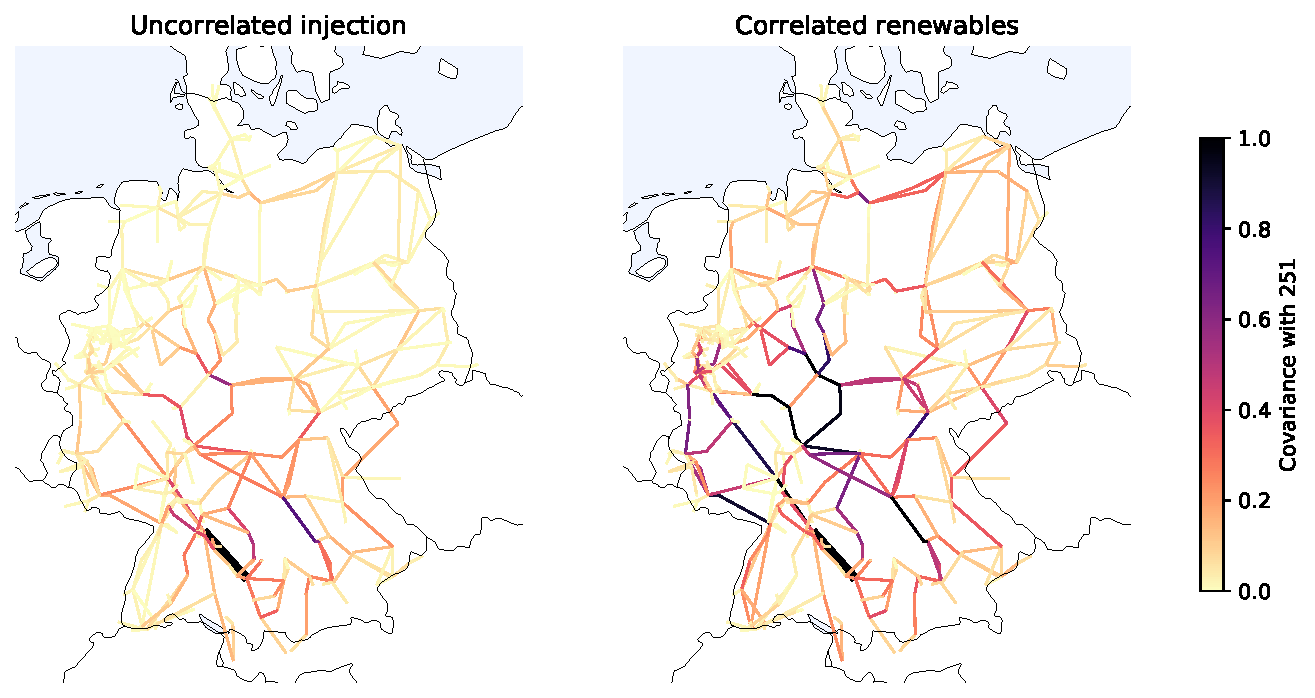
\includegraphics[height=.65\paperheight]{img/flow_correlation_251_iid_and_fullcov.pdf}
    \caption{Covariance relative to line 251.}
    \end{figure}
\end{frame}


\begin{frame}{Correlated flow, daytime}
    \begin{figure}
    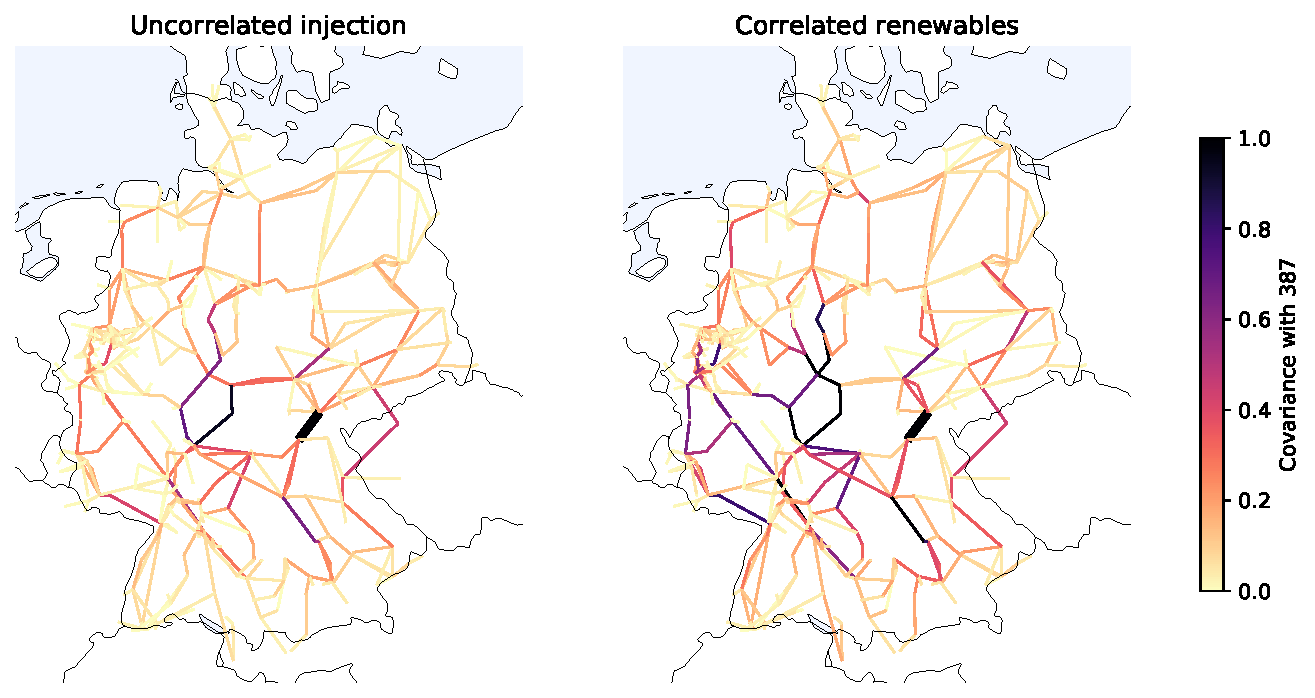
\includegraphics[height=.65\paperheight]{img/flow_correlation_387_iid_and_fullcov.pdf}
    \caption{Covariance relative to line 387.}
    \end{figure}
\end{frame}

\begin{frame}{Long-range correlations}
    \begin{figure}
    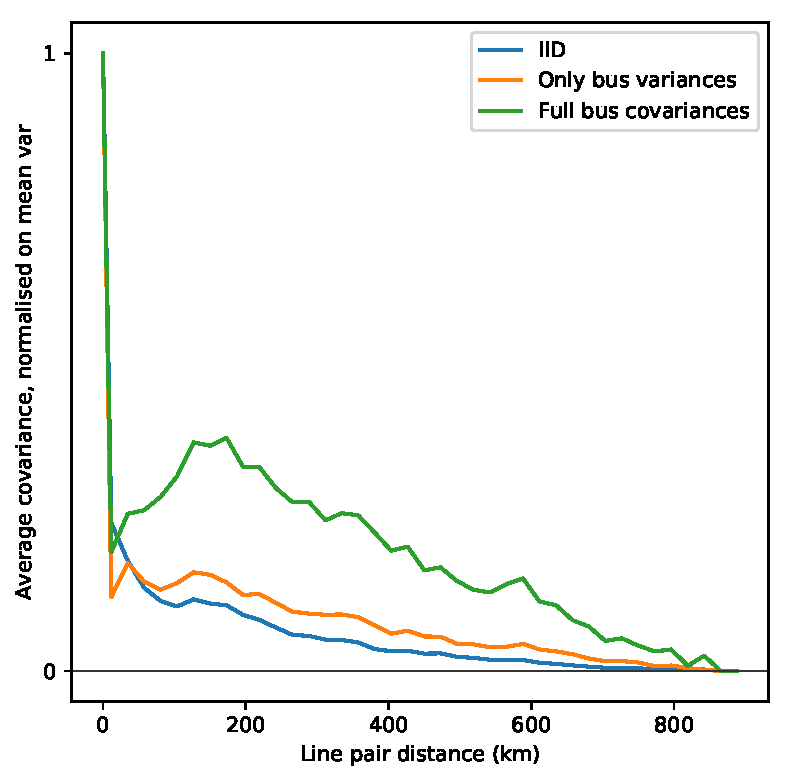
\includegraphics[height=.65\paperheight]{img/line_covariance_vs_line_distance.pdf}
    \caption{Covariances of $10^5$ random line pairs, versus their distance.}
    \end{figure}
\end{frame}

\section{Cascading failures}
\begin{frame}{Cascades}
Flow redistributions cause new failures!
\begin{figure}
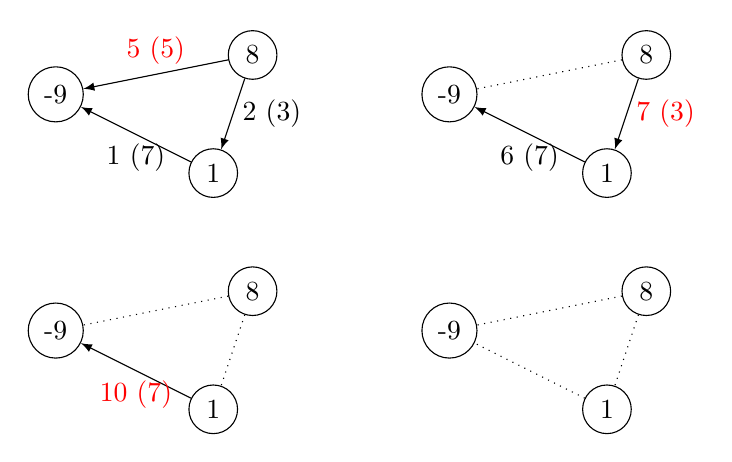
\begin{tikzpicture}[scale=.5]
    \node[draw, circle](b1) at (6,9){8};
    \node[draw, circle](f1) at (1,8){-9};
    \node[draw, circle](l1) at (5,6){1};
    
    
    \draw[-latex] (b1) -- node[midway, right] {2 (3)} (l1);
    \draw[-latex] (l1) -- node[midway, below]{1 (7)} (f1);
    \draw[-latex] (b1) -- node[midway, above]{\color{red}{5 (5)}} (f1);
    
    
    \node[draw, circle](b2) at (16,9){8};
    \node[draw, circle](f2) at (11,8){-9};
    \node[draw, circle](l2) at (15,6){1};
    
    
    \draw[-latex] (b2) -- node[midway, right] {\color{red}{7 (3)}} (l2);
    \draw[-latex] (l2) -- node[midway, below]{6 (7)} (f2);
    \draw[dotted] (b2) --  (f2);
    
    
    \node[draw, circle](b3) at (6,3){8};
    \node[draw, circle](f3) at (1,2){-9};
    \node[draw, circle](l3) at (5,0){1};
    
    
    \draw[dotted] (b3) -- (l3);
    \draw[-latex] (l3) -- node[midway, below]{\color{red}{10 (7)}} (f3);
    \draw[dotted] (b3) --  (f3);
    
    
    \node[draw, circle](b4) at (16,3){8};
    \node[draw, circle](f4) at (11,2){-9};
    \node[draw, circle](l4) at (15,0){1};
    
    
    \draw[dotted] (b4) -- (l4);
    \draw[dotted] (l4) -- (f4);
    \draw[dotted] (b4) --  (f4);
\end{tikzpicture}
\end{figure}
\end{frame}


\plaatjeframe

\begin{frame}{Top 10 risky lines!}
\begin{table}
\begin{tabular}{lrr}
\toprule
line & $\mathbb{P}[|F_l| \geq 1]$ & cascaded \\
\midrule
651 &      9.56 \% &        1 \\
652 &      8.96 \% &        1 \\
411 &      7.06 \% &        1 \\
54  &      6.21 \% &        1 \\
298 &      3.45 \% &       13 \\
473 &      3.13 \% &        1 \\
213 &      2.37 \% &        1 \\
25  &      2.11 \% &        2 \\
645 &      2.02 \% &       32 \\
74  &      1.96 \% &        1 \\
\bottomrule
\end{tabular}
\end{table}
\end{frame}

\begin{frame}{Less risky lines: lower top 50}
\begin{table}
\begin{tabular}{llr}
\toprule
line & $\mathbb{P}[|F_l| \geq 1]$ & cascaded \\
\midrule
459 &  $9.51\cdot 10^{-7}$ &      137 \\
280 &  $7.90\cdot 10^{-7}$ &      185 \\
481 &  $7.61\cdot 10^{-7}$ &      216 \\
337 &  $5.82\cdot 10^{-7}$ &        3 \\
22  &  $3.47\cdot 10^{-7}$ &      125 \\
416 &  $3.12\cdot 10^{-7}$ &      178 \\
144 &  $2.69\cdot 10^{-7}$ &      198 \\
654 &  $1.26\cdot 10^{-7}$ &      175 \\
188 &  $1.02\cdot 10^{-7}$ &      152 \\
18  &  $6.43\cdot 10^{-8}$ &      162 \\
\bottomrule
\end{tabular}

\end{table}
\end{frame}

\section{Conclusions}
\begin{frame}{Conclusions}
\begin{itemize}
\item \textbf{Long-distance correlations} in line currents are \textbf{increased} because of correlated weather.
\item \alert{If an emergent failure occurs, it can \textbf{coincide with} or \textbf{cause} other failures.}
\end{itemize}
\hphantom{x}\\[2em]
\begin{itemize}
\item Complex behaviour of transmission networks arises from simple, \emph{elegant} mathematical structure
\end{itemize}
\end{frame}


{\setbeamercolor{palette primary}{fg=black, bg=black}
\begin{frame}[standout]
  Questions?
\end{frame}
}

\appendix

\section{Appendix}

\begin{frame}{LPF accuracy}
    \begin{figure}
        \centering
        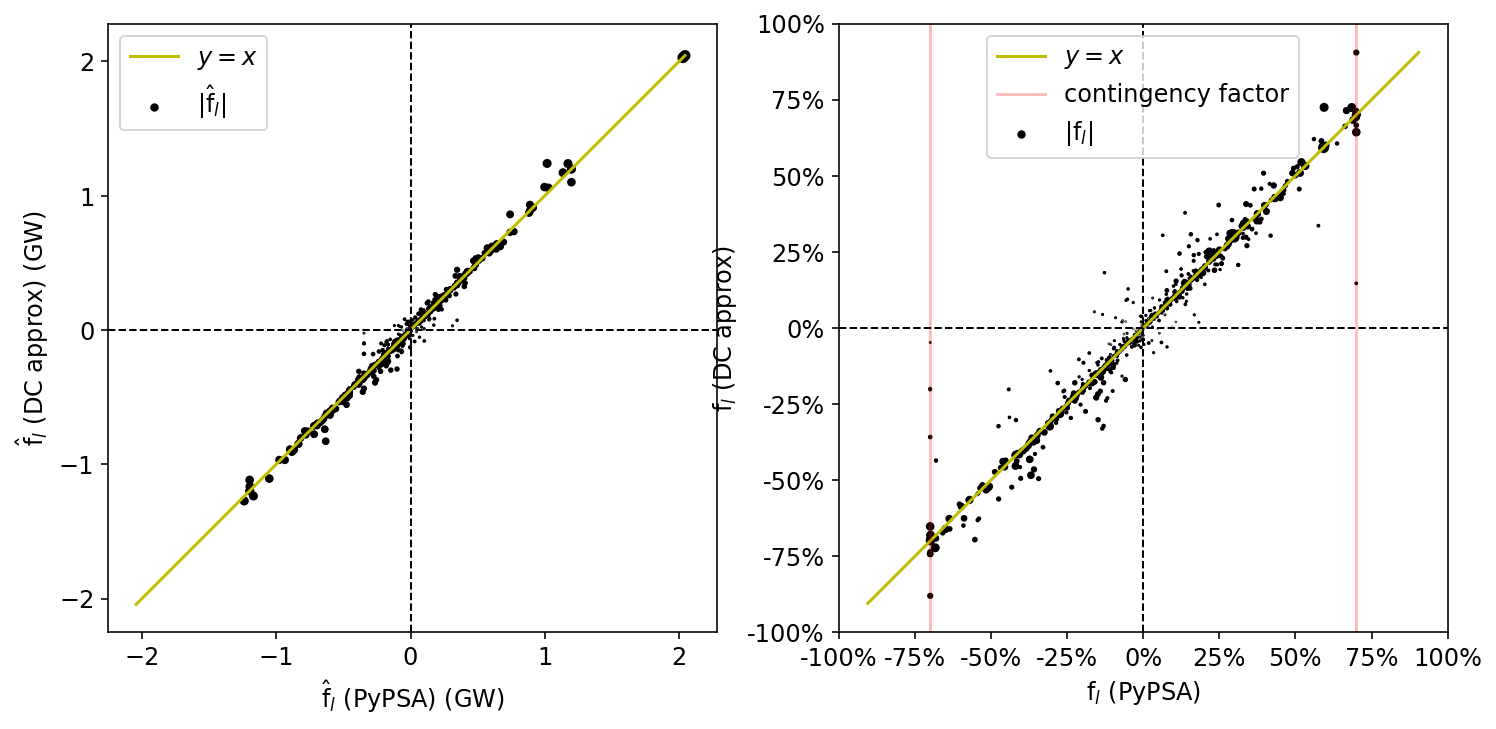
\includegraphics[width=\textwidth]{img/lineflowcorr.png}
        \caption{Line flow (left) and saturation (right) computed using LPF and (non-linear) PF}
    \end{figure}
\end{frame}
\begin{frame}{Solar model}
    \begin{figure}
        \centering
        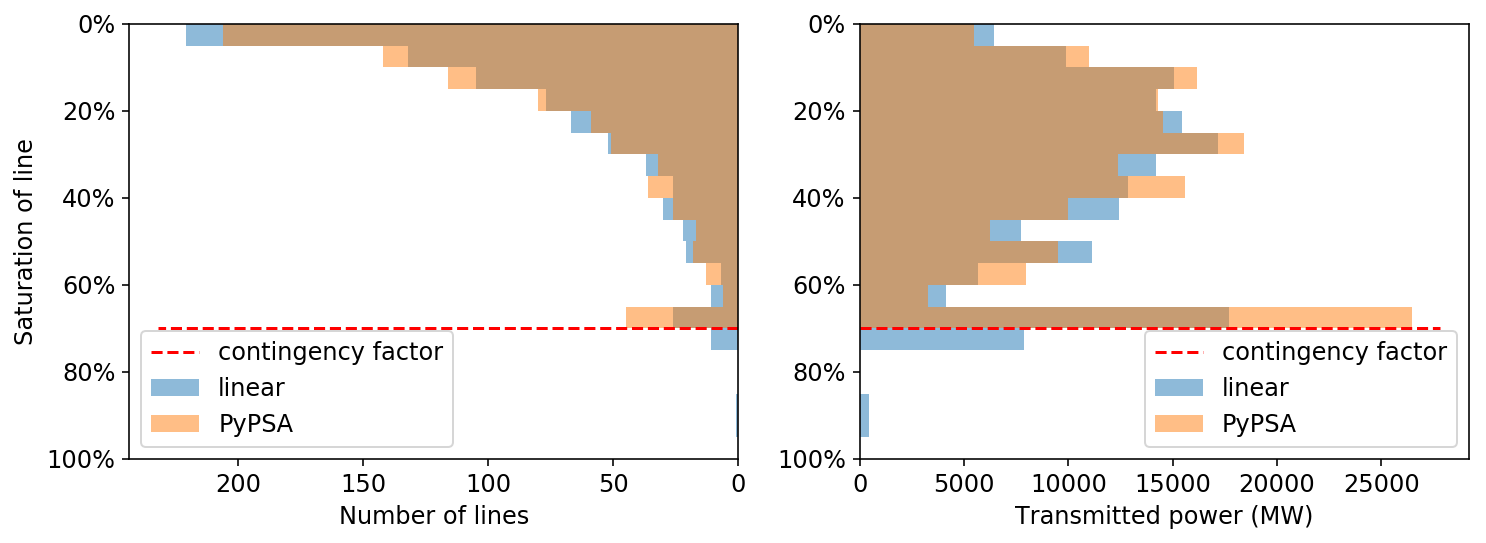
\includegraphics[width=\textwidth]{img/saturationhistrot.png}
        \caption{Histogram of line flow (left) and saturation (right) computed using LPF and (non-linear) PF}
    \end{figure}
\end{frame}

\begin{frame}{Solar model}
    \begin{figure}
        \centering
        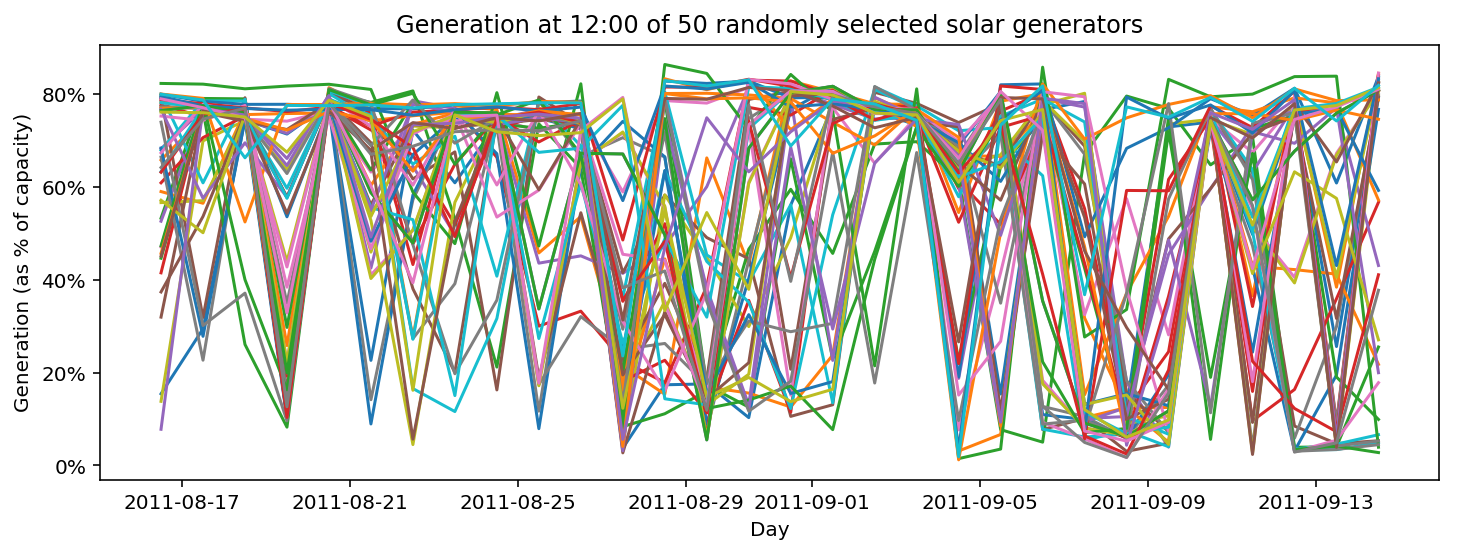
\includegraphics[width=\textwidth]{img/genprofilerandom.png}
        \caption{Daily solar generation at random nodes}
        \label{fig:genprofilerandom}
    \end{figure}
\end{frame}

{
\usebackgroundtemplate{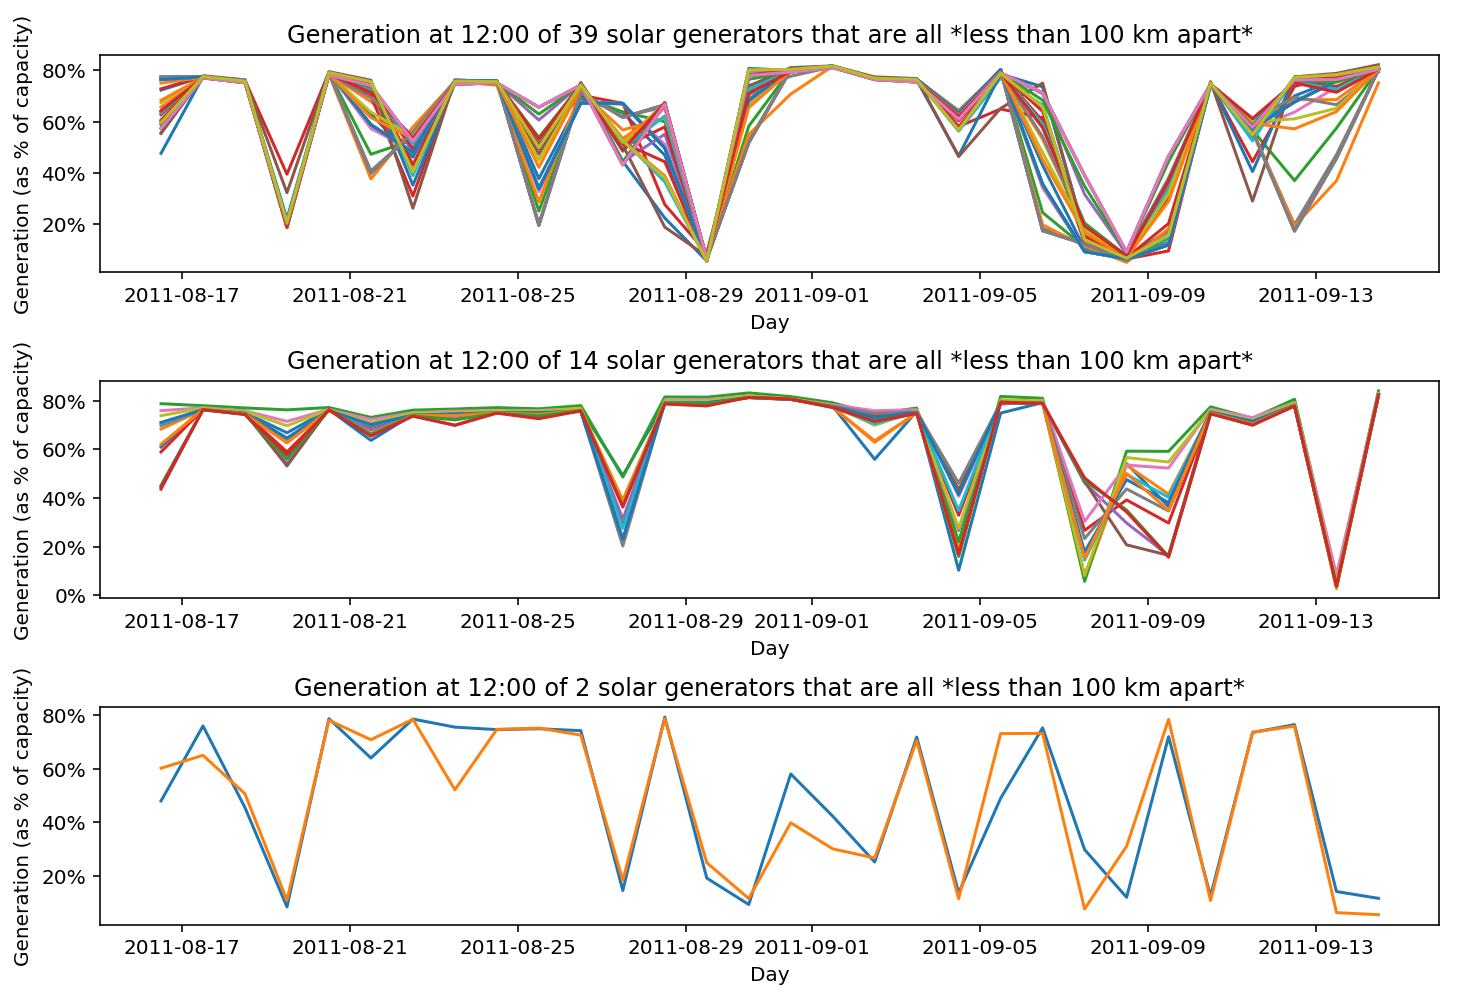
\includegraphics[width=\paperwidth]{img/genprofileclose.png}}
\begin{frame}[plain]
\end{frame}
}

\begin{frame}{ARMA?}
    \begin{figure}
        \centering
        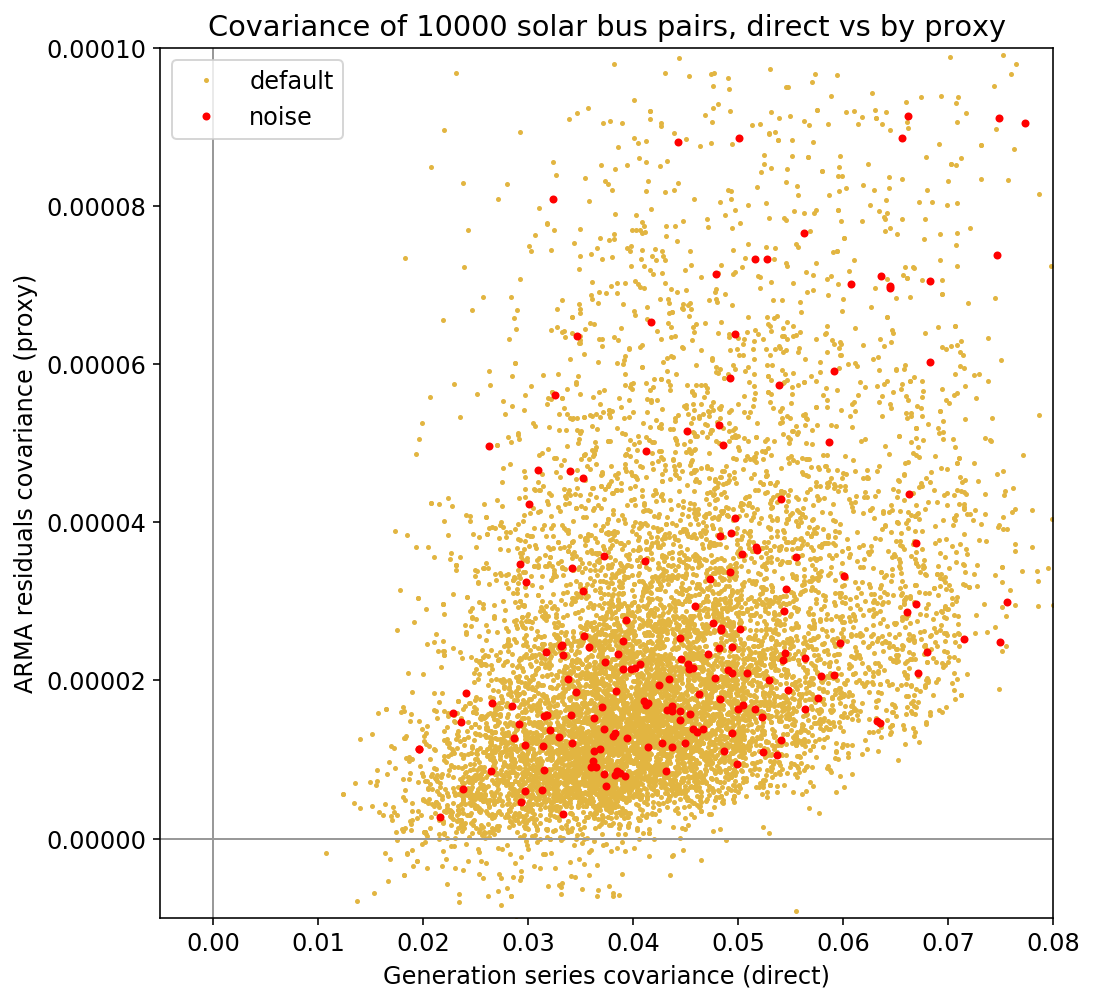
\includegraphics[height=.65\paperheight]{img/cov_direct_vs_proxy_solar.png}
        \caption{Two methods for estimating bus covariances}
    \end{figure}
\end{frame}

{
\usebackgroundtemplate{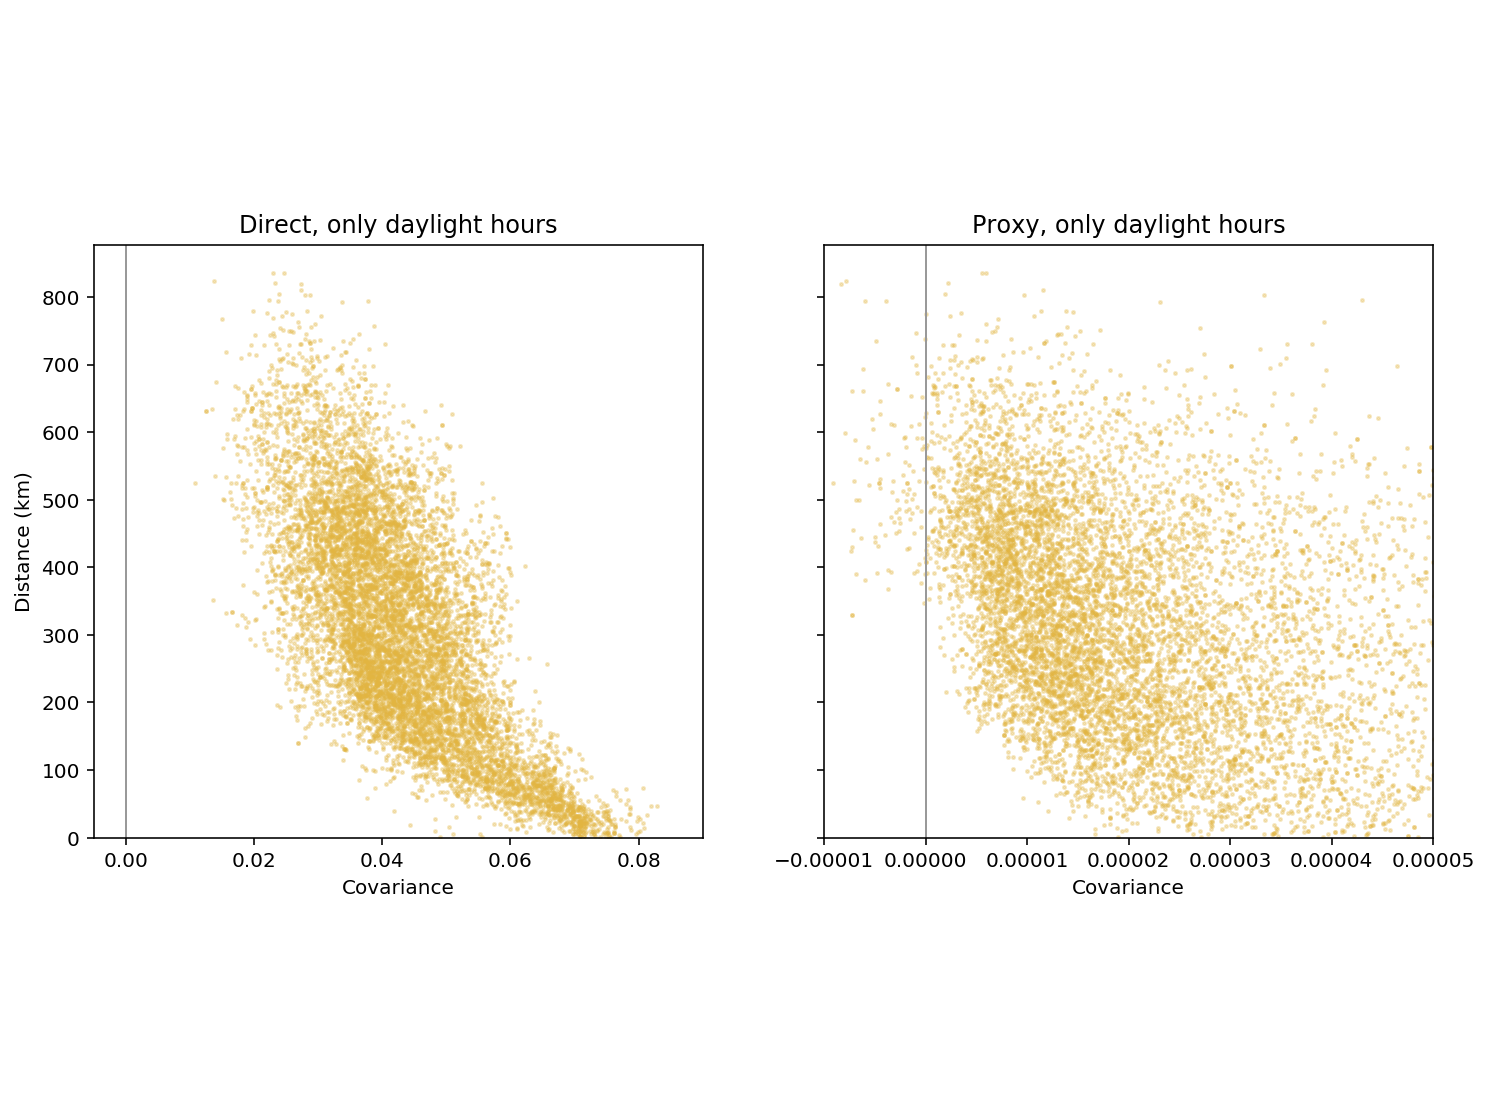
\includegraphics[width=\paperwidth]{img/cov_falloff_solar.png}}
\begin{frame}[plain]
\end{frame}
}

\begin{frame}{ARMA?}
    \begin{figure}
        \centering
        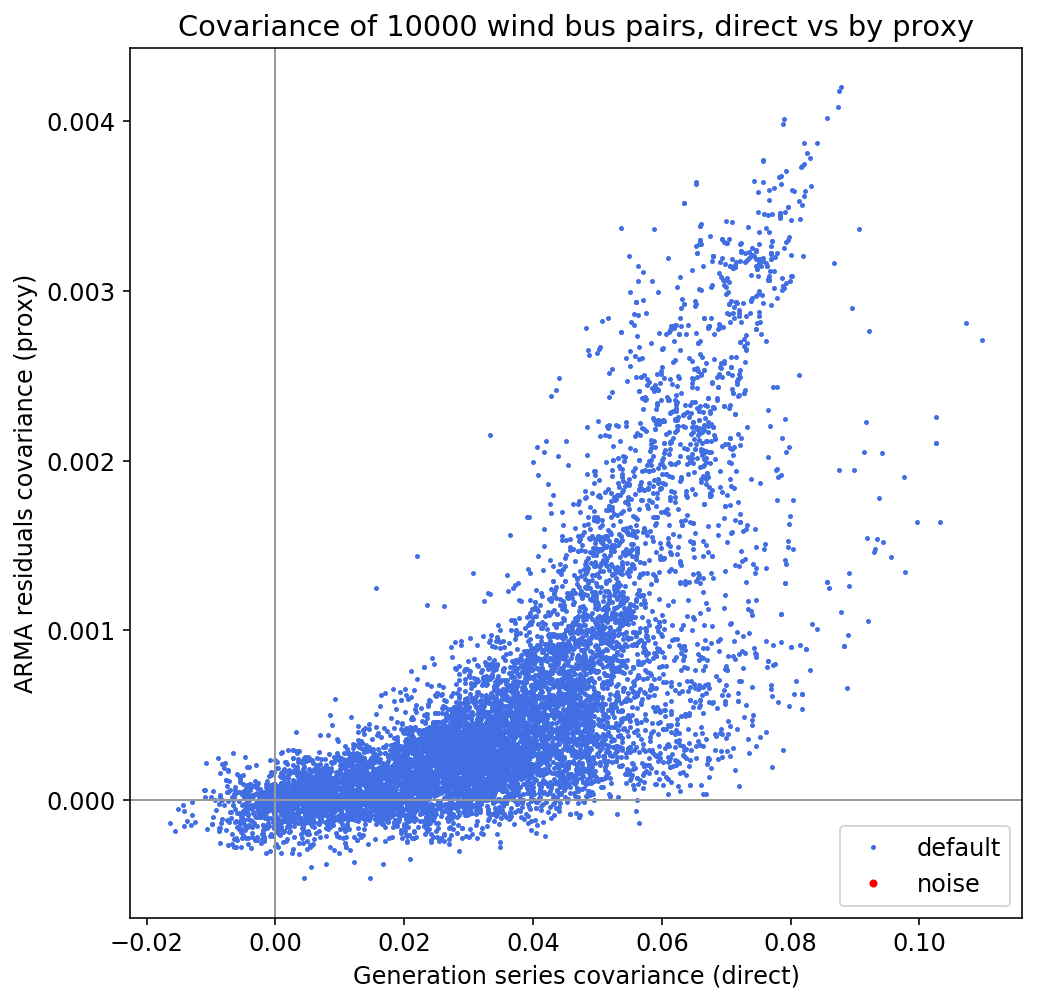
\includegraphics[height=.65\paperheight]{img/cov_direct_vs_proxy_wind.png}
        \caption{Two methods for estimating bus covariances}
    \end{figure}
\end{frame}

{
\usebackgroundtemplate{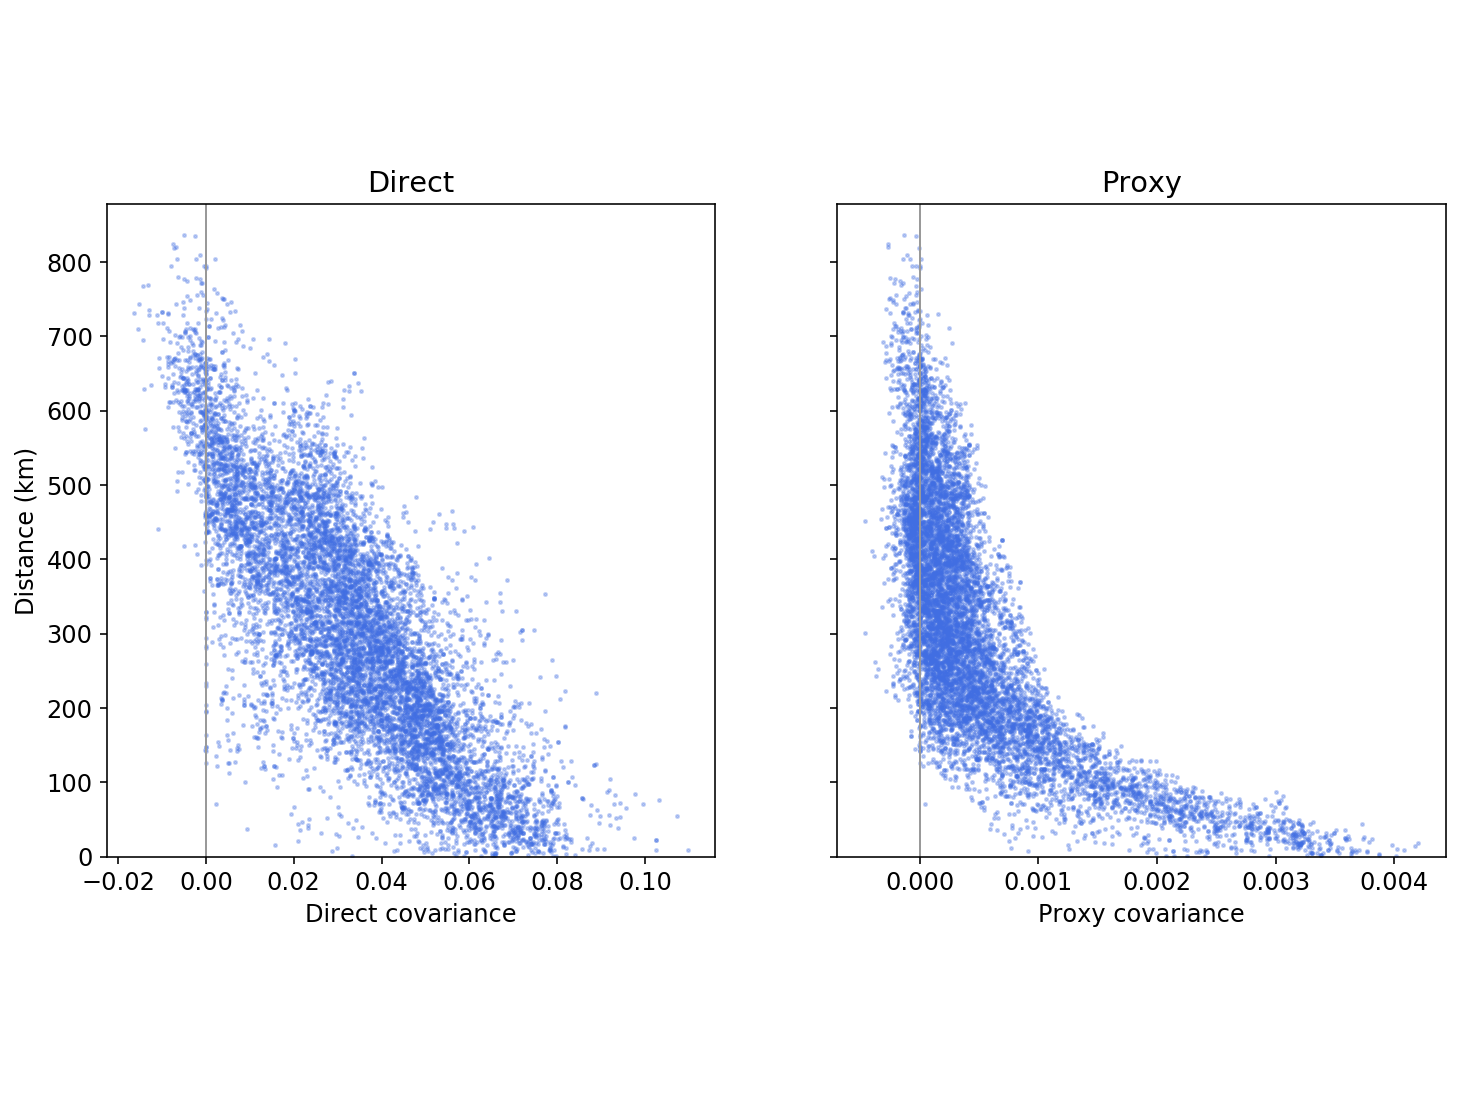
\includegraphics[width=\paperwidth]{img/cov_falloff_wind.png}}
\begin{frame}[plain]
\end{frame}
}

\begin{frame}{Github}
  \begin{center}\href{https://github.com/fonsp/grid-analysis}{github.com/fonsp/grid-analysis}\end{center}
\end{frame}




\end{document}
